\documentclass[10pt,journal,compsoc]{IEEEtran}


\usepackage{booktabs} % For formal tables
\usepackage{xspace}
\usepackage{mathtools}
\usepackage{amsthm}
\usepackage{algorithm}
\usepackage{todonotes}
\usepackage{color}
\usepackage{enumitem}
\usepackage{balance}
\usepackage{flushend}
\usepackage[noend]{algpseudocode}

% These commands are optional
%\acmBooktitle{Transactions of the ACM Woodstock conference}
%\editor{Jennifer B. Sartor}
%\editor{Theo D'Hondt}
%\editor{Wolfgang De Meuter}

\newcommand{\formal}[1]{\textbf{\textsc{#1}}\xspace}
\DeclarePairedDelimiter{\ceil}{\lceil}{\rceil}
\DeclarePairedDelimiter{\floor}{\lfloor}{\rfloor}

\newtheorem{theorem}{Theorem}
\newtheorem{corollary}{Corollary}
\newtheorem{lemma}{Lemma}
\newtheorem{example}{Example}
\newtheorem{definition}{Definition}

\newcommand{\cudpp}{{\tt CUDPP}\xspace}
\newcommand{\megakv}{{\tt MegaKV}\xspace}
\newcommand{\linear}{{\tt Linear}\xspace}
\newcommand{\google}{{\tt GoogleHash}\xspace}
\newcommand{\voter}{{\tt DyHash}\xspace}

\newcommand{\dstwitter}{{\tt TW}\xspace}
\newcommand{\dsreddit}{{\tt RE}\xspace}
\newcommand{\dstpch}{{\tt LINE}\xspace}
\newcommand{\dsali}{{\tt COM}\xspace}
\newcommand{\dsrandom}{{\tt RAND}\xspace}

\newcommand{\xxx}{\textbf{\color{red}{XXX}}\xspace}


\begin{document}
\title{Dynamic Hash Tables on GPUs}


\author{Yuchen~Li, Jing Zhang, Yue Liu, Zheng Lyu, Zhongdong Huang, Jianling Sun
	\IEEEcompsocitemizethanks{
		\IEEEcompsocthanksitem Y. Li is with the School of Information Systems,
		Singapore Management University.
		E-mail: yuchenli@smu.edu.sg
		\IEEEcompsocthanksitem J. Zhang, Y. Liu, Z. Huang and J. Sun are with the College of Computer Science and Technology, Zhejiang University.
		E-mail: \{zhangjing000, liuyue1013, hzd, sunjl\}@zju.edu.cn
		\IEEEcompsocthanksitem Z. Lyu is with the Alibaba Group.
	}%
}

%\numberofauthors{1}
%\author{
%	\alignauthor
%	Yuchen Li$^\dagger$, Jing Zhang, Yue Liu, Zheng Lyu$^*$, Zhongdong Huang, Jianling Sun\\
%	\affaddr{$^\dagger$Singapore Management University},
%	\affaddr{$^*$Alibaba Group},
%	\affaddr{Zhejiang University}
%	\email{$^\dagger$yuchenli@smu.edu.sg, $^*$lvzheng.lz@alibaba-inc.com, \\
%		\{zhangjing000, liuyue1013, hzd, sunjl\}@zju.edu.cn}
%}


\IEEEtitleabstractindextext{%
\begin{abstract}
Hash table, one of the most fundamental data structure,
have been implemented on Graphics Processing Units (GPUs) to accelerate a wide range of data analytics workloads. Most of the existing works focus on the static scenario and try to occupy large GPU device memory for maximizing the insertion efficiency. In many cases, the data stored in the hash table gets updated dynamically and existing approaches takes unnecessarily large memory resources.
One na\"ive solution is to rebuild a hash table (a.k.a rehashing) whenever it is either filled or mostly empty. However, this approach renders significant overheads for rehashing.
In this paper, we propose \emph{DyCuckoo}, a novel dynamic cuckoo hash table on GPUs. 
We devise an efficient resizing strategy for the dynamic scenario without rehashing the entire table and the strategy ensures a guaranteed filled factor.
The strategy trades search performance with resizing efficiency and the tradeoff can be configured by the users.
To further improve efficiency, we further propose a two-layer cuckoo hashing scheme that ensures at most \emph{two} lookups for find and delete opertaions, while still retains similar performance for insertion as that of general cuckoo hash tables. 
Extensive experiments have validated the effectiveness of the proposed design over several state-of-the-art hash table implementations on GPUs. For bounded filled factor, our hash table design achieves up to \xxx speedups over the compared approaches against dynamic workloads. 
\end{abstract}
}

\maketitle
\IEEEdisplaynontitleabstractindextext
\IEEEpeerreviewmaketitle

\section{introduction}
The exceptional advances of General-Purpose Graphics Processing Units (GPGPUs) 
in recent years have completely revolutionized the computing paradigm across multiple fields, including cryptocurrency mining \cite{o2014bitcoin,taylor2013bitcoin}, machine learning \cite{coates2013deep,abadi2016tensorflow}, and database technologies \cite{bakkum2010accelerating,kaldewey2012gpu}.
GPUs bring astonishing computational power that is only available from supercomputers in the past. 
The state-of-the-art commercial GPU equipment (GV100) is capable to operate at the speed of 14.8 TFLOPS for single precision arithmetic and 870 GB/s peak memory bandwidth \footnote{Quadro GV100 launched by NVIDIA in March 2018}. 
Meanwhile, as the computing resources of GPUs continue to explode, it makes rooms for more applications to run on a single GPU equipment concurrently. For example, GV100 is built with 5120 CUDA cores and 32GB device memory. Nevertheless, most GPU programs try to occupy as much resources as possible to maximize their performance individually. 
The egoism renders inefficiency when the GPUs run multiple programs simultaneously. Imagining a number of concurrent programs requesting a total memory size larger than the device memory. Interleaving the program executions leads to redundant data transfers between CPUs and GPUs through PCIe, which is expensive in nature. 

In this paper, we investigate a fundamental data structure, i.e., \emph{hash table}, which has been implemented on GPUs to accelerate numerous applications, ranging from relational hash join \cite{he2008relational,he2009relational,heimel2013hardware}, data mining \cite{pan2011fast,zhou2010parallel,zhong2014medusa},  key value store \cite{zhang2015mega,hetherington2015memcachedgpu,breslow2016horton} and many others \cite{bowers2010parallel,pan2010efficient,garcia2011coherent,niessner2013real,wu2015gpu}. Existing works \cite{alcantara2009real,zhang2015mega,hong2010mapcg,hetherington2015memcachedgpu,breslow2016horton} focus on the static scenario: they know the data size in advance and allocate a sufficiently large hash table to insert all data entries efficiently. In many cases, the data size varies and static allocation leads to poor device memory utilization. To fill this gap, we design a dynamic GPU hash table that adaptively adjusts to the size of active entries in the table. The hash table supports efficient memory management by sustaining a guaranteed \emph{filled factor} of the table when the data size changes. There are two major challenges for maintaining a high filled factor for hash tables on GPUs:

\begin{itemize}
	\item It leads to a smaller hash table size with less distinct keys, hence triggers additional conflicts as multiple threads trying to insert/delete the data, which is particularly expensive under the GPU architecture;
	\item It also means that the table needs to be frequently adjusted to the active data size and it incurs costly rehashing to move the entries to a new table when the old table cannot accommodate the adjusted data. 
\end{itemize}

To overcome the aforementioned challenges, we propose a dynamic cuckoo hash table on GPUs. Cuckoo hashing \cite{pagh2004cuckoo} uses a number of hash functions to provide each key with multiple locations instead of one. When a location is occupied, existing key is relocated to make room for the new one. Existing works \cite{alcantara2009real,alcantara2011building,zhang2015mega,breslow2016horton} have demonstrated great success in speeding up their respective applications by paralleling cuckoo hash on GPUs. 
However, most of these works require the size of a Key-Value (KV) pair to fit a single atomic transaction on GPUs (64 bits wide) to handle conflicts when multiple threads trying to update keys hashed to the same value.
%They also build on inefficient locking mechanisms to handle conflicts, which severely downgrade the performance when high contention occurs. 
In addition, a complete relocation of the entire hash table is required when the data cannot be completely inserted. 
It thus calls for a general hash table design to support larger KV size as well as efficient relocation strategy against dynamic updates.
In this work, we offer two novel designs for implementing dynamic cuckoo hash tables on GPUs. 

First, we propose a voter-based coordination scheme among massive GPU threads to support efficient locking without assuming the size of the key-value pairs.
For each hash value, we allocate a bucket of $b$ locations to store key-value pairs. 
Each thread is assigned to an insertion operation on one key. Instead of immediately acquiring a lock on the corresponding bucket to be updated, a thread will first propose a vote among its warp group and all threads in that same warp collaborate to join the winner thread for its update task. There are three distinguishing advantages for the voter-based coordination: (a) once a conflict is detected on one bucket, instead of spinning, the warp instantly revotes and switches to another bucket; (b) a near-optimal load balancing is achieved as a thread will assist other warp-aligned threads, even when the thread finishes its assigned tasks; (c) locking the bucket exclusively allows to update KV pairs without assuming their length below 64 bits.

Second, we employ the cuckoo hashing scheme with $d$ subtables specified by $d$ hash functions, and introduce a resizing policy to maintain filled factor in a bounded range, while minimizing entries in all subtables relocated at the same time. Insertions and deletions would trigger the hash tables to grow and shrink, if the filled factor falls out of the specified range. 
Our proposed policy only locks one subtable for resizing and it always ensures no subtable can be more than twice as large as any other for handling subsequent resizing efficiently. Meanwhile, the entries in the hash table are distributed so that each subtable has near-equivalent filled factor.
In this way, we drastically reduce the cost of resizing the hash tables and provide better system availability compared with existing works that needs to relocate all data for resizing.
Our theoretical analysis demonstrates the optimality of the scheduling policy in terms of processing updates. 
Empirically, the proposed hash table design is capable to operate efficiently at filled factors exceeding 90\%.

Hereby, we summarize our contributions as follows:
\begin{itemize}
	\item We propose a general dynamic hash table without assuming the size of the key-value pair and devise a novel voter-based coordination scheme to support the locking mechanism under massive GPU threads. 
	\item We introduce an efficient policy to resize the hash tables and our theoretical analysis has demonstrated the near-optimality of the resizing policy.
	\item We conduct extensive experiments on both synthetic and real datasets to showcase the superiority of the proposed approach over several state-of-the-art baselines on GPU hashing. 
	For guaranteed filled factor, our hash table design achieves up to 5x speedups over the baselines against dynamic workloads. The profiling results have also revealed that our approach efficiently leverages GPU resources and demonstrates near-optimal load balancing. 
\end{itemize}

The remaining part of this paper is organized as follows. Section~\ref{sec:pre} introduces the preliminaries and the background on GPUs, followed by the related work in Section~\ref{sec:rel}. Section~\ref{sec:vot} presents our hash table designs as well as the voter-based coordination scheme.  Section~\ref{sec:dyn} introduces our resizing policy against dynamic updates on hash tables. The experimental results are reported in Section~\ref{sec:exp}. Finally, we conclude the paper in Section~\ref{sec:con}. 
\section{preliminaries}\label{sec:pre}
In this section, we first introduce some preliminaries on general hash tables and then present the background on the GPU architecture. 

\begin{table}
	\centering
	\caption{Frequently Used Notations}
	\label{tbl:stat:datasets}
	\begin{tabular}{|c|l|}
		\hline
		$(k,v)$ & a key value pair \\ \hline
		$d$		& the number of hash functions \\ \hline
		$h^i$	& the $i$th hash table \\ \hline
		$|h^i|,n_i,m_i$	& range, table size and data size of $h^i$ \\ \hline
		$wid,l$	& a warp ID and the $l$th lane of the warp \\ \hline
		$\theta$& filled factor of the hash table \\ \hline
		$loc$	& a bucket in the hash table \\ \hline
	\end{tabular}
\end{table}

\subsection{Hash Table}
A hash table is a fundamental data structure to store KV pairs $(k,v)$ and the value could refer to either the actual data or a reference to the data.
The hash table offers the following functionalities: \formal{insert}$(k,v)$ - stores $(k,v)$ in the hash table; \formal{find}$(k)$ - given $k$ returns the associated values if they exist, and NULL otherwise; and \formal{delete}$(k)$ - removes existing KVs that match $k$ if they present in the table.

Given a hash function with range $0 \ldots h-1$, collisions must happen when we insert $m>h$ keys into the table. There are many schemes to resolve collisions: linear probing, quadratic probing, chaining and etc. Contrary to these schemes, cuckoo hashing \cite{pagh2004cuckoo} guarantees a worst case constant complexity for \formal{find} and \formal{delete},  and an amortized constant complexity for \formal{insert}. A cuckoo hash uses multiple (i.e., $d$) hash tables with independent hash functions $h^1,h^2,\ldots,h^d$ and stores a KV in \emph{one} of the hash tables. When inserting a $(k,v)$, we store the pair to $loc=h^1(k)$ and terminate if there is no element at this location. Otherwise, if there exists $k'$ such that $h^1(k')=loc$, $k'$ is evicted and will be reinserted into another hash table, e.g., $loc'=h^2(k')$.
We repeat this process until an empty location is encountered.

For a hash table with the hash function $h^i$, $|h^i|$ is defined to be the number of unique hash values for $h^i$ and $n_i$ to be the total memory size allocated for the hash table.
A location or a hash value for $h^i$ is represented as $loc = h^i_j$ where $j \in [0,|h^i|-1]$.
If the occupied space of the hash table is $m_i$, the filled factor of $h^i$ is denoted as $\theta_i = m_i / n_i$.

\subsection{GPU Architecture}

\begin{figure}[t]
	\centering
	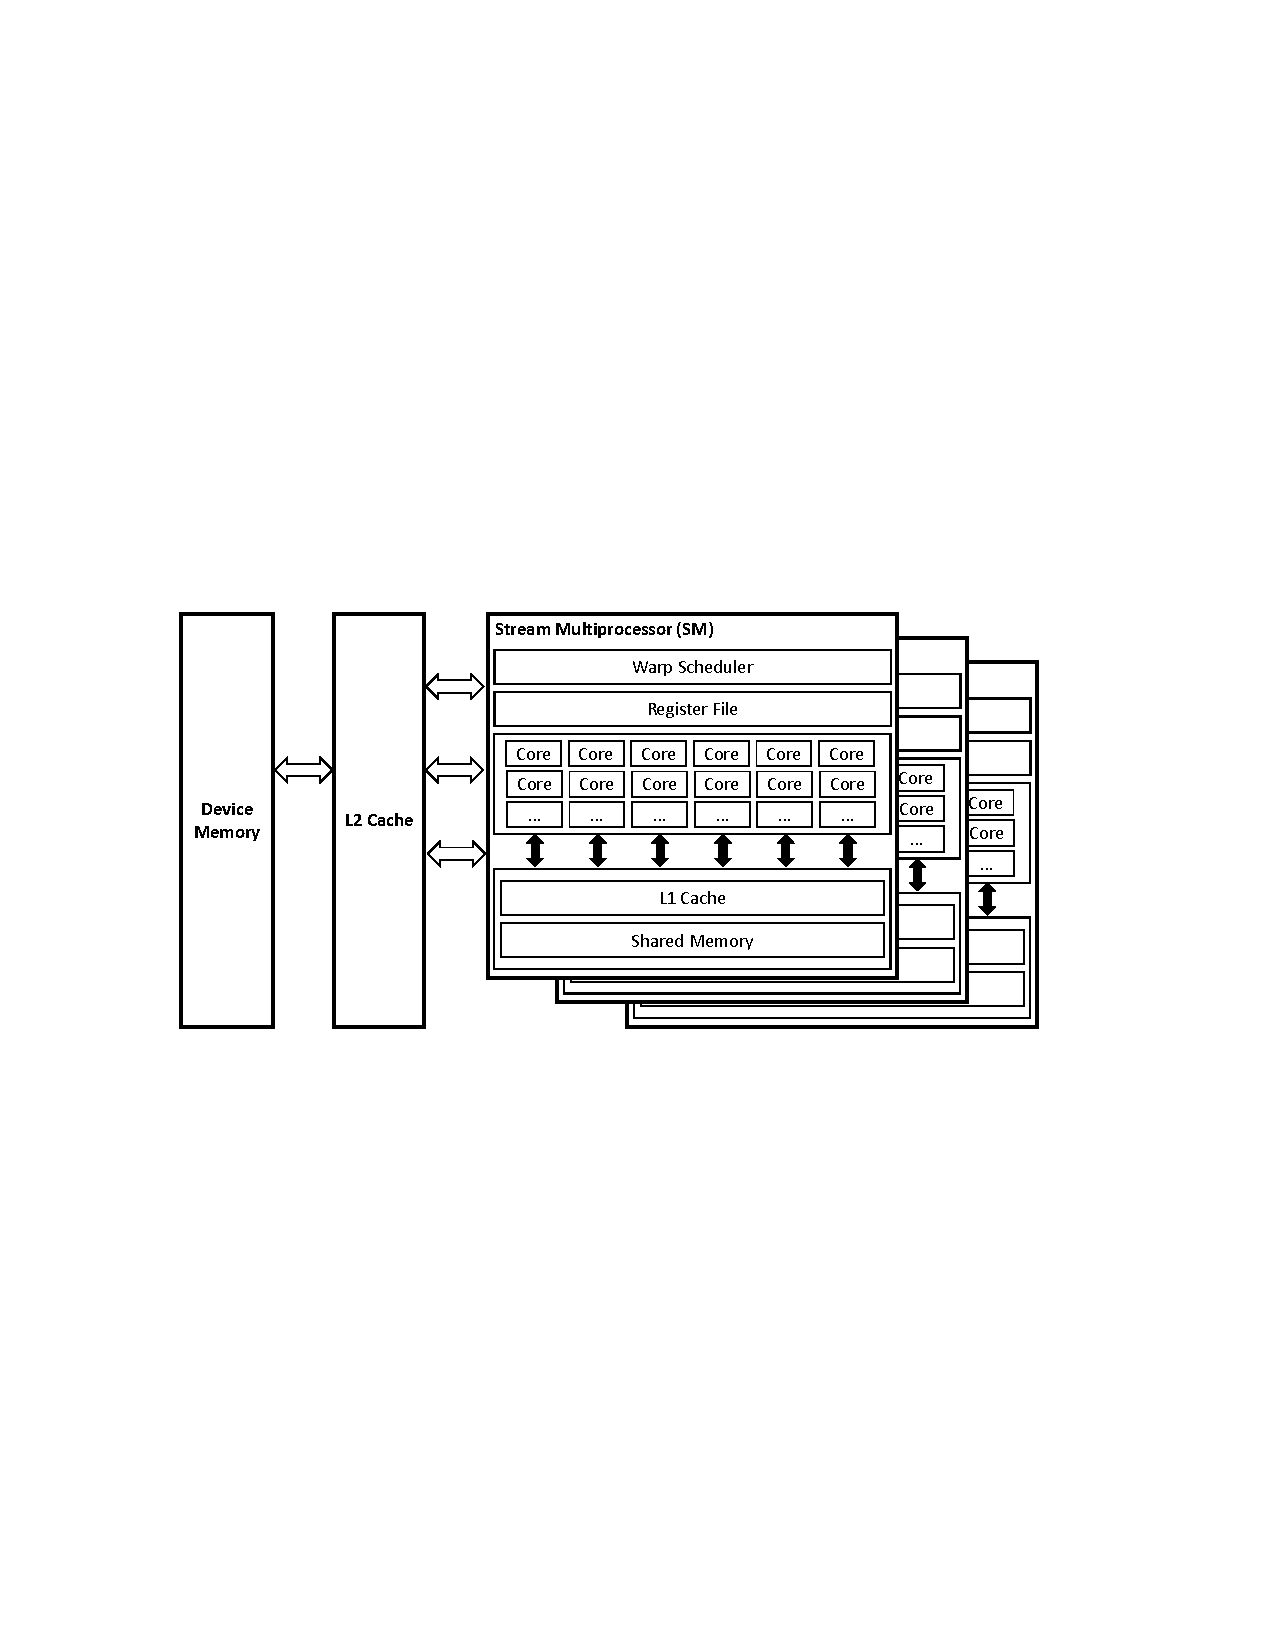
\includegraphics[width=0.5\textwidth]{fig/GPU-arch.pdf}
	\caption{Layout of an NVIDIA GPU architecture}
	\label{fig:arch}
\end{figure}

We focus on introducing the background of NVIDIA GPU architecture in this section due to its popularity and wide adoption of the CUDA programming language. 
It is noted that our proposed approaches are not unique to NVIDIA GPUs and can be implemented on other GPU architectures as well. Figure~\ref{fig:arch} presents a high-level layout of a NVIDIA GPU. An application written in CUDA executes on GPUs through invoking the \emph{kernel} function. The kernel is organized as a number of \emph{thread blocks}, and one block executes all its threads on a \emph{streaming multiprocessor}, which contains a number of CUDA cores as depicted in the figure. Within a block, threads are divided into \emph{warps} of 32 threads each. 
A CUDA core executes the same instruction of a warp in a lockstep\footnote{Although the latest Volta architecture supports independent thread scheduling \cite{},
	it is still more efficient to run with the lockstep execution model.}.
Each warp runs independently but can collaborate through different memory types discussed as the following.  

%\vspace{1mm}\noindent\textbf{Memory Hierarchy.} Compared CPUs, GPUs are built with large register files to enable massive parallelism. 
%For example, NVIDIA GTX 1080 GPUs feature 256KB of register files for each SM. Furthermore, the shared memory, which has similar performance with the L1 cache, can be programmed within a block to facilitate efficient local memory access inside a SM.
%The L2 cache is shared among all SMs to speedup memory access to the device memory. The device memory has the largest capacity and the lowest bandwidth in the GPU memory hierarchy.

%GPUs offer an significant better data accessing throughputs than CPUs for two major reasons. 
%First,the device memory has high memory bandwidth, often an order of magnitude faster than RAM.
%Second, GPUs effectively hide memory access latency by warp switching. When a warp is blocked by memory accesses, other warps whose next instruction has its operands ready are eligible to be scheduled for execution. With sufficient threads launched, memory stalls can be minimized or even eliminated \cite{zhang2015mega}.
%Thus, the fast data accessing performance makes GPUs an ideal accelerator for data intensive applications such as hash tables. 

%Data is transferred between CPUs and GPUs (or between two GPU devices) via the PCIe link (Gen 3), which has been the bottleneck of many data-intensive applications \cite{zhang2015mega,kaldewey2012gpu,zhang2013omnidb}. In recent years, there have been many innovations proposed to reduce the overhead of the data transfer, from overlapping PCIe transfer with kernel execution to using hardware acceleration such as PCIe Gen 4 and NVlink \cite{thompto2016power9}. Nonetheless, we omit the discussion on how to minimize this data transfer cost since it is orthogonal to designing an efficient hash table on \emph{one} GPU device.

\vspace{1mm}\noindent\textbf{Optimizing GPU Programs.}
When programming a GPU device, there are several important guidelines to harness GPUs' massive parallelism.
\begin{itemize}
	\item \emph{Minimize Warp Divergence.} Threads in a warp will be serialized if they execute different instructions. To enable maximum parallelism, one needs to minimize branching statements executed within a warp.  
	\item \emph{Coalesced Memory Access.} Warps have a wide cache line size (128 bytes for NVIDIA GPU). The threads are better off to read consecutive memory locations for fully utilizing the device memory bandwidth, otherwise to trigger multiple random accesses for a single read instruction by a warp. 
	\item \emph{Control Resource Usage.} Registers and shared memory are valuable resources to enable fast local memory accesses. Nevertheless, each SM has limited resources (GTX 1080 has 98 KB shared memory and 256KB register files per SM). Overdosing register files or shared memory leads to reduced parallelism on a SM.  
	\item \emph{Atomic Operations.} When facing thread conflicts, an improper locking implementation leads to serious performance degradation. One can leverage the native support of atomic operations \cite{sanders2010cuda} on GPUs to carefully resolve the conflicts and minimize thread spinning.
\end{itemize}
\section{related works}\label{sec:rel}
Alcantara \textit{et al.} present a seminar work on GPU-based cuckoo hashing to accelerate computer graphics workloads \cite{alcantara2009real}. 
This work has inspired a number of applications from diverse fields. Wu \textit{et al.} investigate the use of GPU-based cuckoo hashing for
on-the-fly model checking \cite{wu2015gpu}. A proposal of accelerating the nearest neighbor search is presented in \cite{pan2010efficient}. 
Due to the success of cuckoo hashing on GPUs, the implementation of \cite{alcantara2009real} has been adopted in the CUDPP library\footnote{https://github.com/cudpp/cudpp}.
To improve from \cite{alcantara2009real}, stadium hash is proposed in \cite{khorasani2015stadium} to support out-of-core GPU parallel hashing. However it uses double hashing which needs to rebuild the entire table for any deletions.  
Zhang \textit{et al.} propose another efficient design of GPU-based cuckoo hashing, named MegaKV, 
to boost the performance for KV store \cite{zhang2015mega}. 
Subsequently, Horton table \cite{breslow2016horton} improves the efficiency of \formal{find} over MegaKV by trading with the cost of introducing a KV remapping mechanism.
Meanwhile, in the database domain, several SIMD hash table implementations have been proposed to facilitate relation join and graph processing, including cuckoo hash \cite{ross2007efficient} and linear probing \cite{zhong2014medusa}. 

It is noted that the aforementioned works focus on the static case: the size of data that needs to be hashed is known in advance. Thus, the static designs would prepare a sufficiently large memory to store the hash table. In this way, the hash table operations are fast since the collision rarely happens. However, the static approach wastes memory resources and, to some extent, it prohibits data from other applications to coexist on the device memory. 
This motivates us to develop a dynamic hash table on GPUs that actively makes adjustments according to the data size. 
In this paper, we propose a dynamic cuckoo hash table on GPUs, which maintains high filled factor to minimize memory footprint. In order to support efficient concurrent hash updates, we introduce a novel voter-based coordination scheme which reduces thread conflicts. Experimental results have revealed that the proposed solution could achieve competitive or even better performance than the state-of-the-art static hash tables on GPUs, while utilizing significantly less device memory. 

To the best of our knowledge, there is only one existing work for building dynamic hash tables on GPUs \cite{ashkiani2018dynamic}.
This proposed approach presents a concurrent linked list structure, called \emph{slab list}, to construct the dynamic hash table with \emph{chaining}. 
However, parallel chaining incurs two major issues. 
First, it could frequently invoke concurrent memory allocation requests, especially when the data keeps inserting. Efficient concurrent memory allocation is difficult to implement under the GPU architecture due to its massive parallelism. Although a dedicated memory management strategy is proposed in \cite{ashkiani2018dynamic} to alleviate this allocation cost, it is not transparent to other applications. More specifically, the dedicated allocator still needs to reserve a large piece of memory in advance to prepare for efficient dynamic allocation, and the occupied space cannot be readily accessed by other concurrent applications. 
Second, the chaining approach has a lookup time of $\Omega(log(log(m)))$ for some KVs with high probability. This not only results in degraded performance for \formal{find}, but also triggers more overheads in resolving conflicts when multiple \formal{insert} and \formal{delete} operations occur at the same key.
In contrast, the cuckoo hashing table adopted in this work guarantees $\Theta(1)$ worst case complexity for \formal{find} and \formal{delete}, 
$O(1)$ amortized \formal{insert} performance. We do not introduce extra complication in implementing our own version of memory manager and only reply on the default memory allocator provided by CUDA. 
\section{Dynamic Hash Table}\label{sec:dyn}
In this section, we propose the resizing strategy against dynamic hash table updates on GPUs. We first present the hash table design in Section~\ref{sec:dyn:has}.
Subsequently, the resizing strategy is introduced in Section~\ref{sec:dyn:resize}.
In section~\ref{sec:dyn:distribute}, we discuss how to distribute the KV pairs for better load balancing with theoretical guarantees. 
Finally, we present how to efficiently rehash and relocate the data after the tables have been resized in Section~\ref{sec:dyn:rehash}. 

\subsection{Hash Table Structure}\label{sec:dyn:has}
Following cuckoo hashing \cite{pagh2004cuckoo}, we build $d$ hash tables with $d$ unique hash functions: $h^1,h^2,\ldots,h^d$. 
In this work, we use a set of simple universal hash function such as $h^i(k) = (a_i\cdot k + b_i \mod p) \mod |h^i|$.
$a_i,b_i$ are random integers, $p$ is a large prime.
Note that the proposed approaches in this paper also apply to other hash functions as well. 
There are three major advantages for adopting cuckoo hashing on GPUs. 
First, it avoids chaining by inserting the elements into alternative locations if collision happens. As discussed in Section~\ref{sec:rel}, 
chaining presents several issues which are not friendly to the GPU architecture.  
Second, to lookup a KV pair, one only needs to search $d$ locations specified by $d$ unique hash functions. 
Thus, the data could be stored contiguously in the same location and enable the preferred coalesced memory access. 
Third, cuckoo hashing can maintain high filled factor, which is ideal for memory saving in the dynamic scenario. 
For $d=3$, cuckoo hashing achieves over $90\%$ filled factor and still processes \formal{insert} operations efficiently \cite{fotakis2005space}.

\begin{figure}[t]
	\centering
	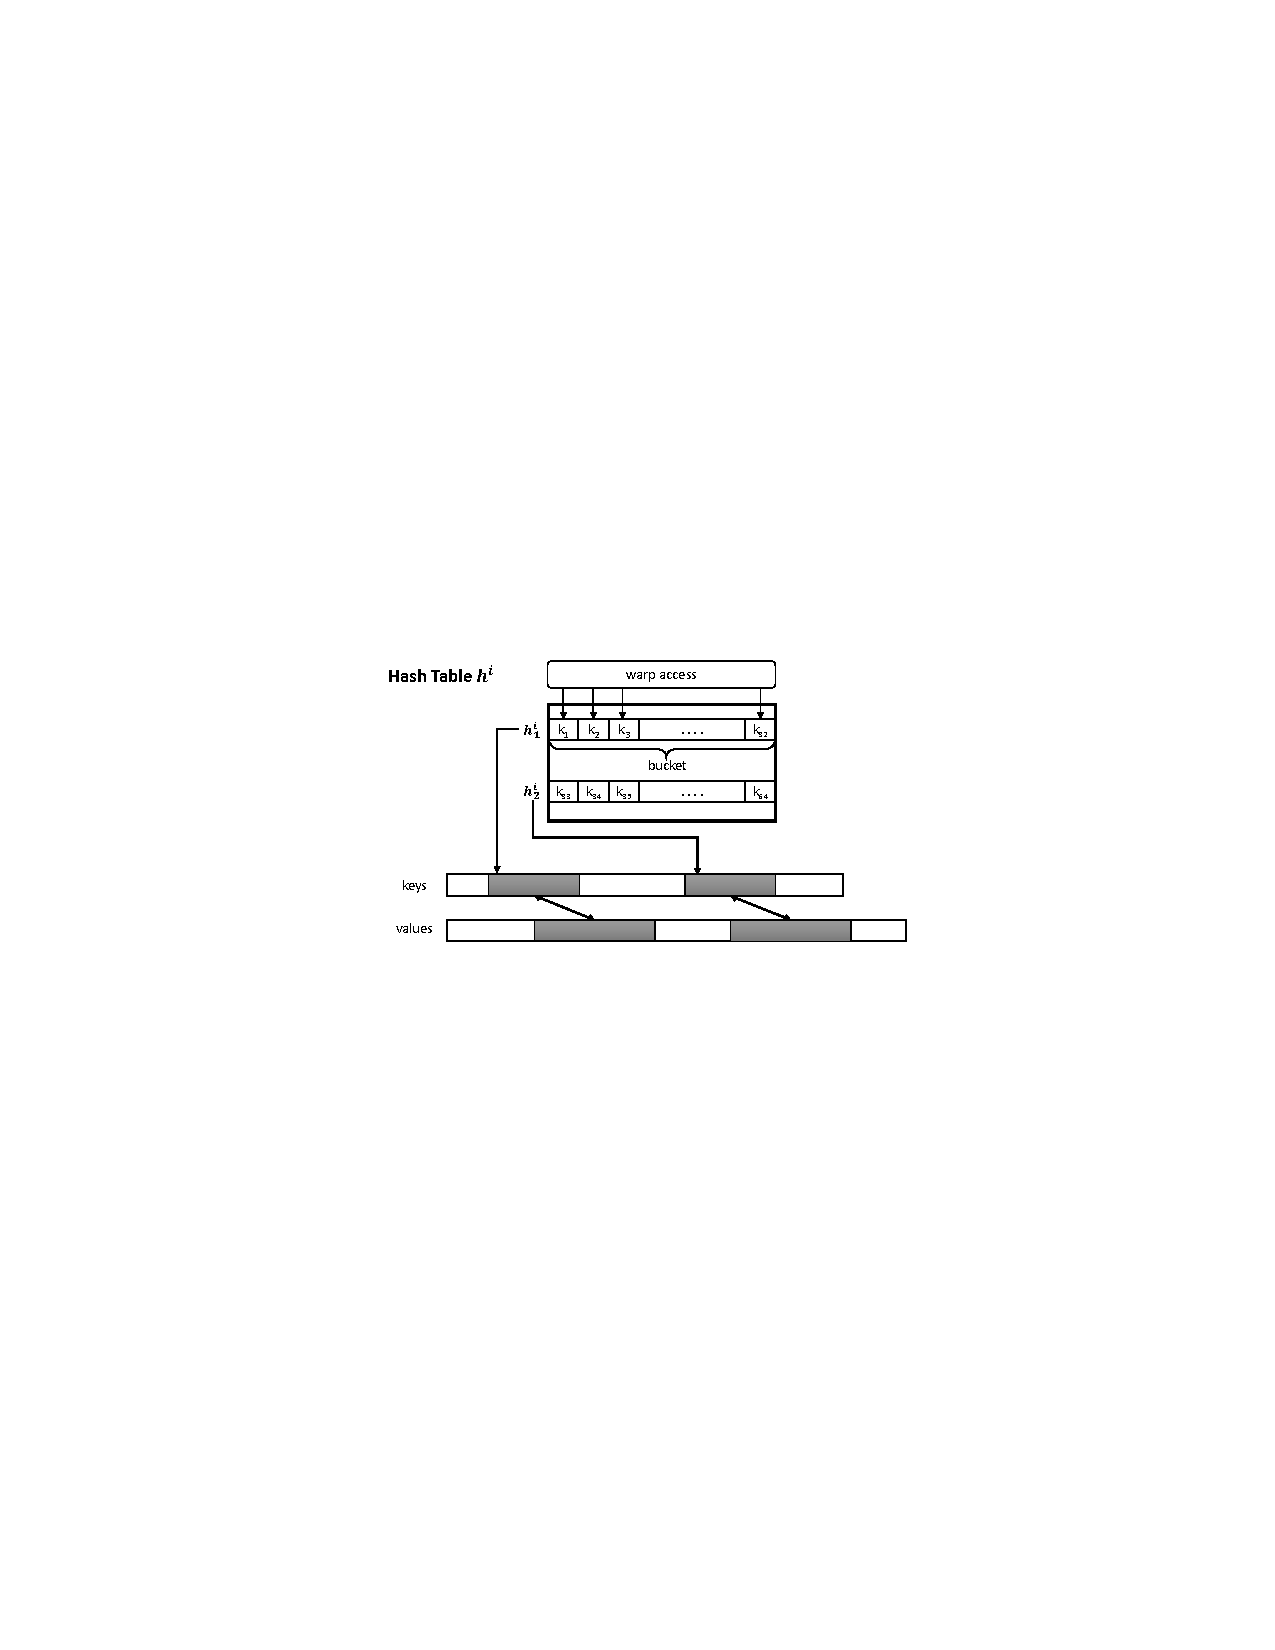
\includegraphics[width=0.45\textwidth]{fig/Hashtable.pdf}
	\caption{The hash table structure}
	\label{fig:hashtable}
\end{figure}

Figure~\ref{fig:hashtable} depicts the design of a single hash table $h^i$ on GPUs. 
Assuming the keys are 4-byte integers. A bucket of 32 keys, which are all hashed to the same value $h^i_j$, are stored consecutively in the memory. 
The design of buckets maximizes the utilization of memory bandwidth in GPUs. 
Consider the L1 cache line size is 128 bytes, only a single access is required when one warp is assigned to access a bucket. 
The values associated with the keys in the same bucket are also stored consecutively but in a separate array.   
In other words, we use two arrays to store the keys and the values respectively.
The values could take much larger memory space than the keys. 
Thus, storing keys and values separately avoid the overhead of memory access when accessing the values are not necessary, 
e.g., finding a nonexistent KV pair or deleting a KV pair. 

For keys having size larger than 4 bytes, a simple strategy is to store less KV pairs in a bucket. Suppose the keys are 8-bytes, a bucket can then accommodate 16 KV pairs. 
Furthermore, we lock the entire bucket exclusively for a warp to perform insertion/deletion using intra warp synchronization primitives. Thus, we do not limit ourselves to supporting KV pairs with only 64 bits. 
In the worst case, a key taking 128 bytes occupy one bucket alone, which is unnecessarily large in practice.

\subsection{Structure Resizing}\label{sec:dyn:resize}
To efficiently utilize GPU device memory, we resize the hash tables when the filled factor falls out of the desired range, e.g., $[\alpha,\beta]$.
One possible strategy is to double or half all hash tables and to then rehash all KV pairs. However, this simple strategy renders poor memory utilization and 
excessive overheads for rehashing. First, doubling the size of the hash tables results in filled factor immediately cut to half, while downsizing the hash tables to half the size followed by rehashing could only be efficient when the filled factor is significantly low (e.g., $40\%$), both of which scenarios are not resource friendly. Second, rehashing all KV pairs is expensive and it hurts the performance stability for most of the streaming applications since the entire hash table is subject to locking. 

We propose an alternative strategy, illustrated in Figure~\ref{fig:resize}. 
Given $d$ hash tables depicted in Figure~\ref{fig:resize},
we always double the smallest subtable or chop the largest subtable into half for upsizing or downsizing respectively, when filled factor falls out of $[\alpha,\beta]$. 
In other words, no subtable will be more than double the size as others. The strategy implies that we do not need to lock all hash tables and only to resize one, thus achieving better performance stability compared with the aforementioned simple strategy. 

\vspace{1mm}
\noindent\textbf{Filled factor analysis:}
Assuming there are $d'$ hash tables with size $2n$, $d-d'$ tables with size $n$ and the current filled factor $\theta$, 
one upsizing process when $\theta > \beta$ lowers the filled factor to $\frac{\theta\cdot(d+d')}{d+d'+1} \geq \frac{\beta \cdot d}{d+1}$.  
Since the filled factor is always lower bounded by $\alpha$, we can deduce that $\alpha < \frac{d}{d+1}$.
Apparently, a higher lower bound can be achieved by adding more hash tables, while it leads to less efficient \formal{find} and \formal{delete}. 
We allow the user to configure the number of hash tables to trade off memory and query processing efficiency. 

\begin{figure}[t]
	\centering
	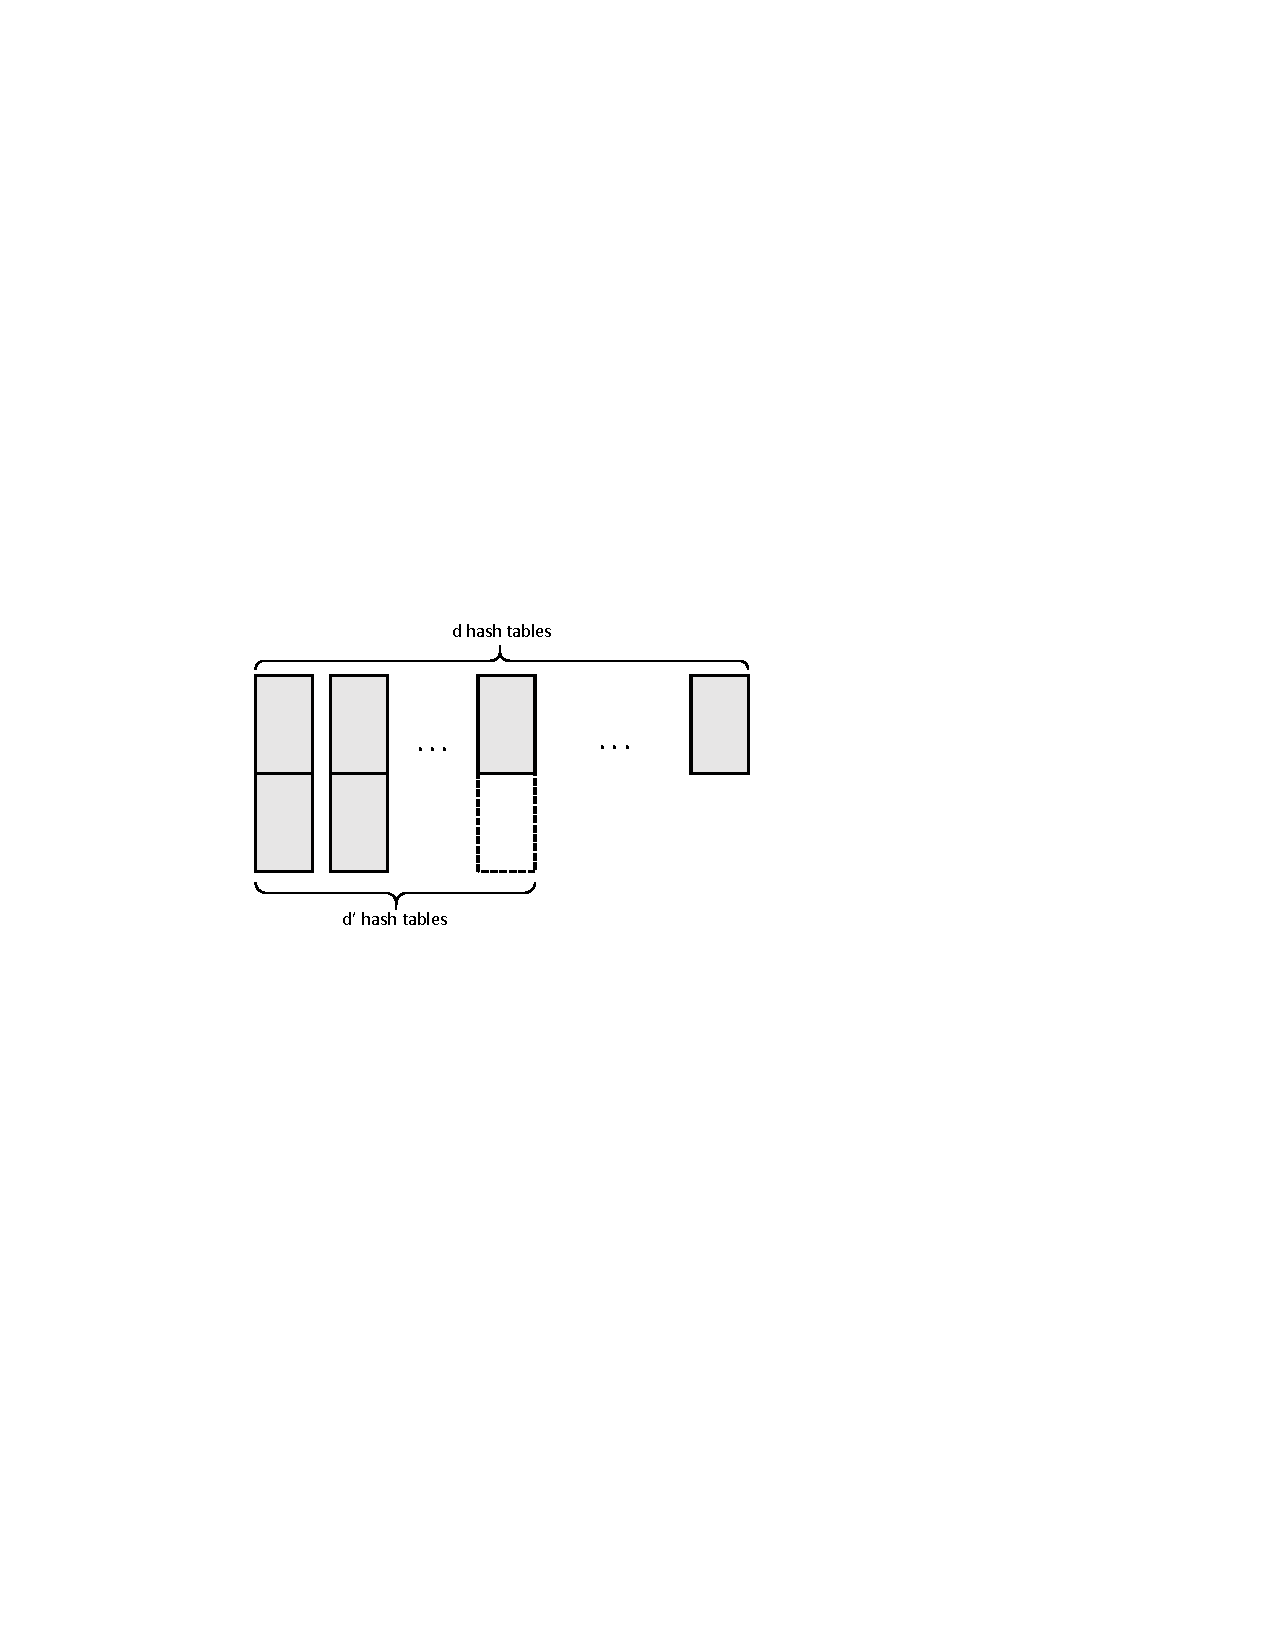
\includegraphics[width=0.35\textwidth]{fig/MultiTable.pdf}
	\caption{Resizing strategy}
	\label{fig:resize}
\end{figure}
\subsection{KV distribution}\label{sec:dyn:distribute}
Given a set of KV pairs to insert in parallel, it is critical to distribute the KV pairs among the hash tables in a way such that the hash collisions are minimized for reducing the corresponding thread conflicts. We have the following theorem to guide us for distributing the KV pairs. 

\begin{theorem}\label{them:balance}
	The amortized conflicts for inserting $m$ unique KV pairs to $d$ hash tables is minimized when $\binom{m_1}{2}/n_1 = \ldots = \binom{m_d}{2}/n_d$. 
	$m_i$ and $n_i$ denote the elements inserted to table $i$ and the size of table $i$ respectively.  
\end{theorem}
\begin{proof}
	It is noted that the amortized insertion complexity of cuckoo hash is $O(1)$. Thus, similar to balls and bins analysis, the expected number of conflicts occurred for inserting $m_i$ elements in table $i$ is estimated as $\binom{m_i}{2}/n_i$. Minimizing the amortized conflicts among all hash tables can be modeled as the following optimization problem:
	\begin{equation}\label{eq:conflict-min}
	\begin{array}{ll@{}ll}
	\min_{m_1,\ldots,m_d \geq 0} & \sum_{i=1,\ldots,d} \binom{m_i}{2}/n_i \\
	\text{s.t.} & \sum_{i=1,\ldots,d} m_i = m
	\end{array}
	\end{equation}
	To solve the optimization problem, we establish an equivalent objective function:
	\begin{align*}
	\min \sum_{i=1,\ldots,d} \frac{\binom{m_i}{2}}{n_i} \Leftrightarrow \min \log(\frac{1}{d}\sum_{i=1,\ldots,d} \frac{\binom{m_i}{2}}{n_i})
	\end{align*}
	By Jensen's inequality, the following inequality holds:
	\begin{align*}
	\log(\frac{1}{d}\sum_{i=1,\ldots,d} \frac{\binom{m_i}{2}}{n_i}) \geq \frac{1}{d}\sum_{i=1,\ldots,d}\log(\frac{\binom{m_i}{2}}{n_i})
	\end{align*}
	where the equality holds when $\binom{m_i}{2}/n_i = \binom{m_j}{2}/n_j$ $\forall i,j = 1,\ldots,d$ and we obtain the minimum.
\end{proof}

According to our resizing strategy, one hash table can only be as twice large as the other tables. 
This implies the filled factors of two tables are equal if they have the same size, i.e., $\theta_i = \theta_j$ if $n_i = n_j$, 
while $\theta_i \simeq \sqrt{2}\cdot \theta_j$ if $n_i = 2n_j$. 
Thus, larger tables should have a higher filled factor. 
Guided by Theorem~\ref{them:balance},
we employ a randomized approach: 
a KV pair $(k,v)$ will be firstly assigned to table $i$ with a probability proportional to $n_i/\binom{m_i}{2}$ to ensure the distribution of KVs.

\subsection{Rehashing}\label{sec:dyn:rehash}
Whenever the filled factor falls out of the desired range, rehashing relocates the KV pairs after one of the hash table is resized. An efficient relocation process maximizes the utilization of GPU device memory bandwidth and minimizes thread conflicts. 
We discuss two scenarios for rehashing: \emph{upsizing} and \emph{downsizing}. Both scenarios are processed in one single kernel. 

\begin{figure}[t]
	\centering
	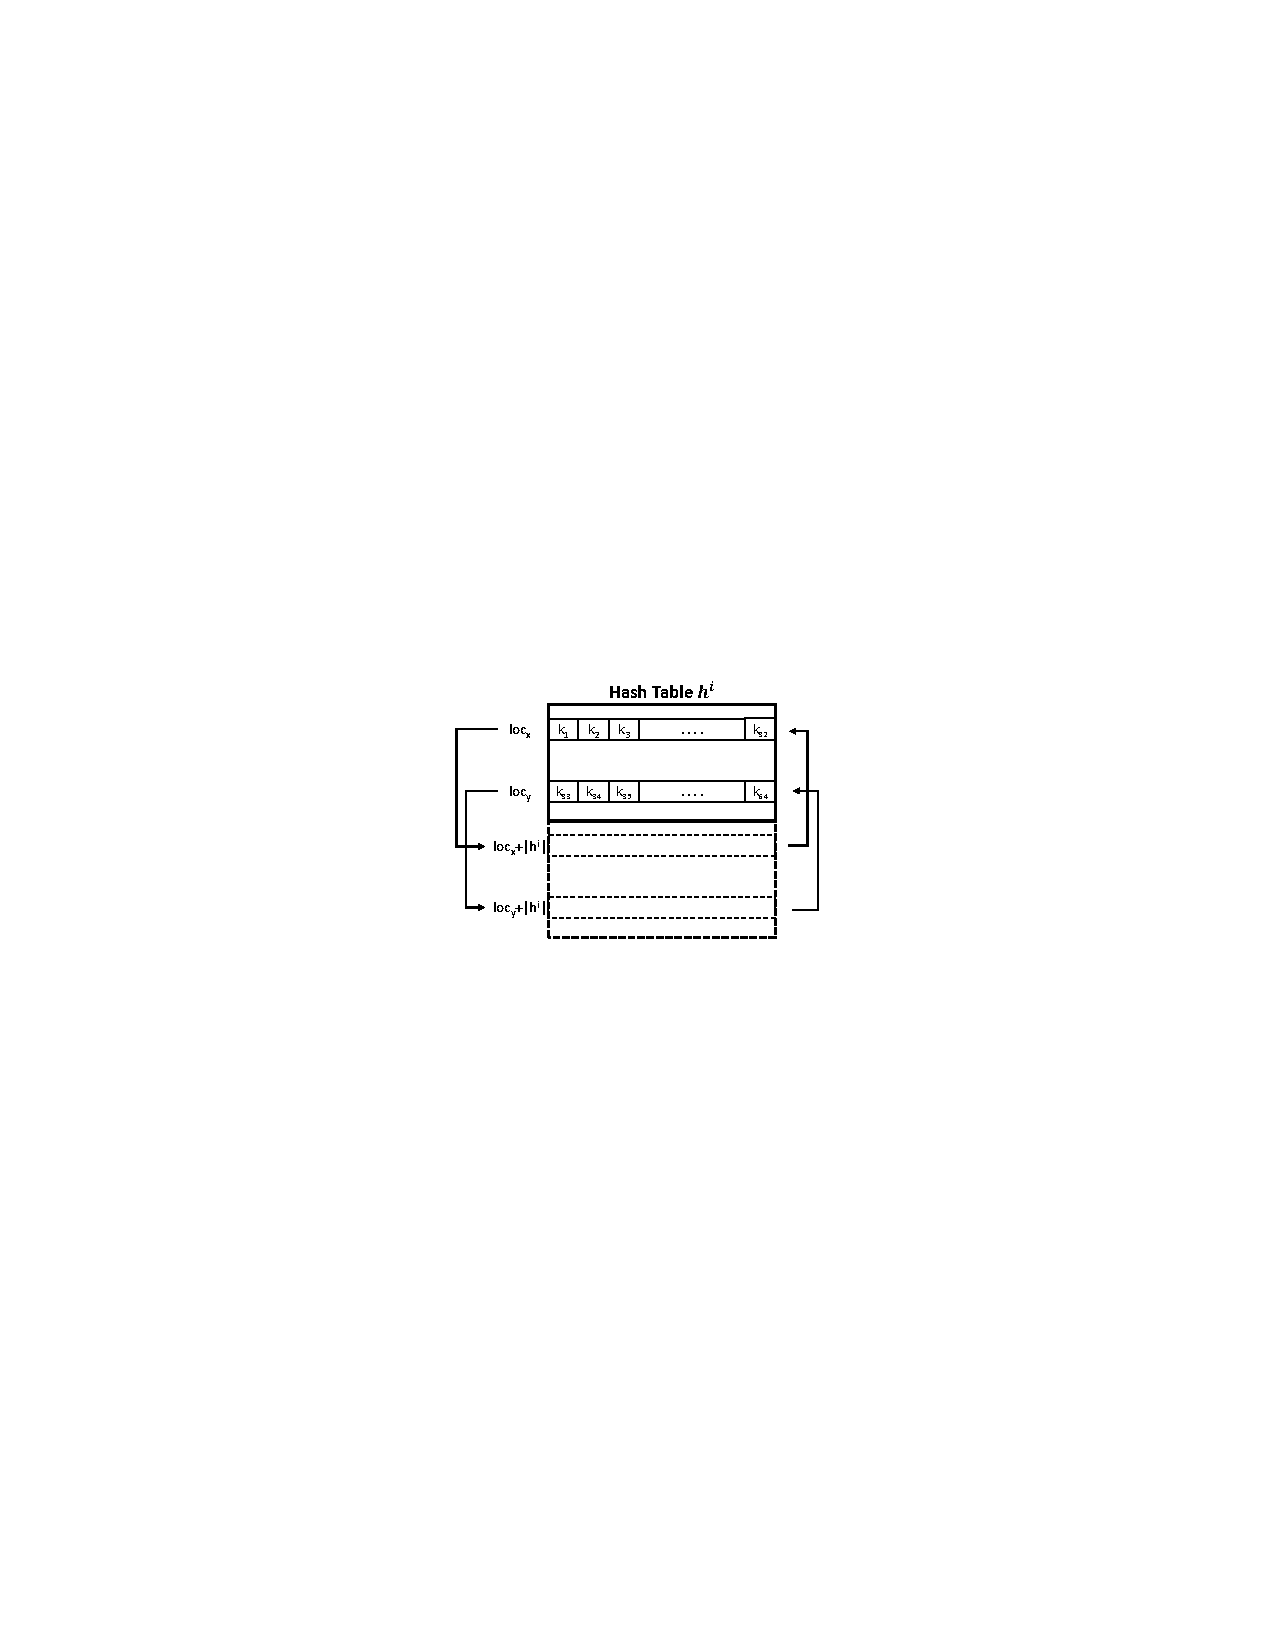
\includegraphics[width=0.3\textwidth]{fig/Upsize.pdf}
	\caption{Illustration for upsizing and downsizing.}
	\label{fig:upsize}
\end{figure}
\vspace{1mm}\noindent\textbf{Upsizing.} 
We introduce a conflict-free rehashing strategy for the upsizing scenario. 
Figure~\ref{fig:upsize} presents an illustration for upsizing a hash table $h^i$. 
As we always double the size for $h^i$, 
a KV pair which originally resides in bucket $loc$ could be rehashed to bucket $loc+|h^i|$ or stay in the original bucket. 
With this observation, we assign a warp for rehashing all KV pairs in bucket to fully utilize the cache line size. 
Each thread in the warp corporately takes a KV pair in the bucket and relocates the KV pair if necessary.
Moreover, the rehashing does not trigger any conflict since KV pairs from two distinct buckets before upsizing cannot be rehashed to the same bucket.  
Thus, the locking of a bucket is not required and we can make use of the full device memory bandwidth for the upsizing process.  

Note that after upsizing hash table $h^i$, its filled factor $\theta_i$ is cut to half, which could break the balancing condition emphasized in Theorem~\ref{them:balance}. Nevertheless, we use the sampling strategy for subsequent KV insertions, where each insertion is allocated to table $i$ with a probability proportional to $n_i/\binom{m_i}{2}$, to recover the balancing condition. In particular, $m_i$ remains the same while $n_i$ doubles after upsizing, the scenario leads to double the probability of inserting subsequent KV pairs to $h^i$. 


\vspace{1mm}\noindent\textbf{Downsizing.}
Downsizing the hash table $h^i$ is a reverse process of upsizing $h^i$. We note that there is always room to relocate KV pairs in the same table for upsizing. 
In contrast, downsizing may rehash some KV pairs to other hash tables, especially when $\theta_i > 50\%$.
Since the KV pairs located in $loc$ and $loc+|h^i|$ are hashed to $loc$ in the new table, there could be cases the KV pairs exceeds the size of a single bucket. 
Hence, we first assign a warp to accommodate KV pairs that can fit the size of a single bucket. Similar as upsizing, it does require locking since there will be no thread conflict on any bucket. 
For the remaining KV pairs which cannot fit in the downsized table, called residuals, we insert them into other subtables.
To make sure no conflict occurs between inserting residuals and processing the downsizing subtable, which are both executed in a single kernel, we exclude the downsizing subtable when inserting the residuals. 
Take an example when we have three subtables and one of them is being downsized. 
We only insert the residuals to the remaining two subtables. 


%To safeguard the balancing condition, we devise a different rehashing strategy for downsizing. 
%For all KV pairs in bucket $loc \geq |h^i|/2$ for table $i$ to be downsized, we assign a thread to rehash and reinsert a KV pair using Algorithm~\ref{algo:insert}. 
%In this way, we achieve the balancing condition at the expense of locking a bucket when reinserting a KV pair. 

\vspace{1mm}\noindent\textbf{Complexity Analysis.}
Given a total of $m$ elements in the hash tables, upsizing/downsizing rehashes at most $m/d$ KV pairs. 
For inserting/deleting these $m$ elements, the number of rehashes is bounded by $2m$. 
Thus, the amortized complexity for inserting $m$ elements is still $O(1)$.

\subsection{Hash Table Structure}\label{sec:vot:has}
\begin{figure}[t]
	\centering
	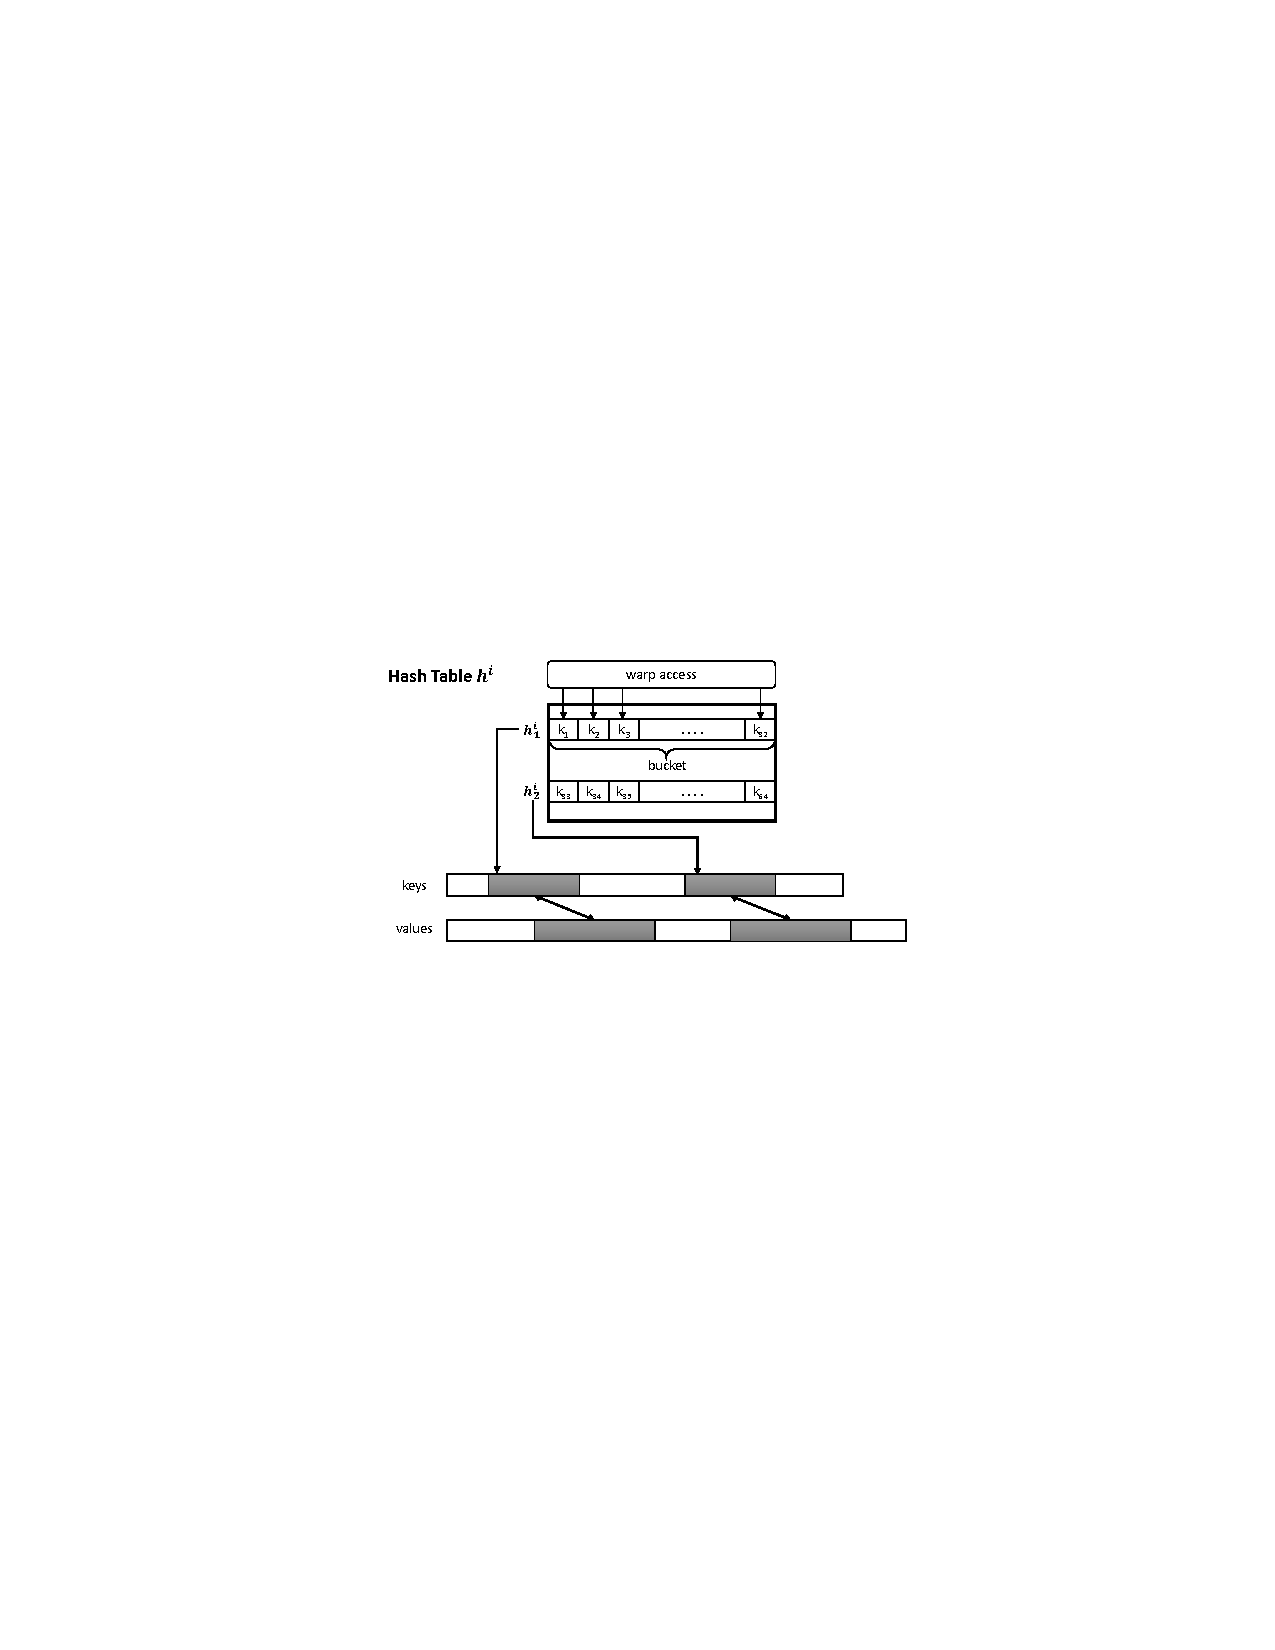
\includegraphics[width=0.45\textwidth]{fig/Hashtable.pdf}
	\caption{The hash table structure}
	\label{fig:hashtable}
\end{figure}

\section{Voter-based GPU Cuckoo Hash}\label{sec:vot}
In this section, we first present a overview of the hash table structure and pinpoint a number of important design objectives in Section~\ref{sec:vot:has}.
Subsequently, in Section~\ref{sec:vot:con}, we give details on how to perform updates with the \emph{voter} coordination, i.e., \formal{find}, \formal{insert} and \formal{delete}, for the case where hash table resizing is not required. 
We leave how to handle the fully dynamic scenario in Section~\ref{sec:dyn} for further discussions. 


Adopted from cuckoo hashing \cite{}, we build $d$ hash tables with $d$ unique hash functions: $h^1,h^2,\ldots,h^d$. 
In this work, we use a set of simple universal hash function such as $h^i(k) = (a_i\cdot k + b_i \mod p) \mod |h^i|$.
$a_i,b_i$ are random integers, $p$ is a large prime.
There are three major advantages for adopting cuckoo hashing on GPUs. 
First, it avoids chaining by inserting the elements into alternative locations if collision happens. As discussed in Section~\ref{sec:rel}, 
chaining present several issues which are not friendly to the GPU architecture.  
Second, to lookup a KV pair, one only needs to search $d$ locations specified by $d$ unique hash functions. 
Thus, the data could be stored contiguously in the same location and thus enable the preferred coalesced memory access. 
Third, cuckoo hashing can maintain high filled factor, which is ideal for memory saving in the dynamic scenario. 
For $d=3$, cuckoo hashing achieves over $90\%$ filled factor and still process \formal{insert} operations efficiently \cite{fotakis2005space}.

Figure~\ref{fig:hashtable} depicts the design of a single hash table $h^i$ on GPUs. 
Assuming the keys are 4-byte integers. A bucket of 32 keys, which are all hashed to the same value $h^i_j$, are stored consecutively in the memory. 
The design of buckets maximizes the utilization of memory bandwidth in GPUs. 
Since the cache line size is 128 bytes, only a single memory load is required when one warp is assigned to access a bucket. 
The values associated with the keys in the same bucket are also stored consecutively but in a separate array.   
In other words, we use two arrays to store the keys and the values respectively.
The values could take much larger memory space than the keys. 
Thus, storing keys and values separately avoid the overhead of memory access when accessing the values are not necessary, 
e.g., finding a nonexistent KV pair or deleting a KV pair. 


\begin{algorithm}[t]
	\begin{algorithmic}[1]
		\State $found \gets \emptyset$
		\For{$i=0,\ldots,d-1$}
		\State $loc \gets h^i(k)$
		\State $found \gets ballot(loc[l].key == k)$
		\If{$found \neq \emptyset$}
		\State \Return $loc[l]$
		\EndIf
		\EndFor
		\State \Return false
	\end{algorithmic}
	\caption{\textbf{Find}(lane $l$, warp $wid$, key $k$)}\label{algo:find}
\end{algorithm}

\subsection{Parallel Hash Table Operations}\label{sec:vot:con}
In the reminder of this session, we discuss how to utilize GPUs' threads to execute hash table operations in parallel.
Following existing works \cite{alcantara2009real,zhang2015mega,breslow2016horton}, we assume the \formal{find}, \formal{insert} and \formal{delete} operations are batched and each batch only contains one type of operations. A batch with mixed type of operations can also be supported but the semantic is ambiguous. 



\vspace{1mm}\noindent\textbf{Find.} It is relative straightforward to parallelize \formal{find} operations since only read access is required. 
Given a batch of size $m$, we launch $w$ warps in total (which means launching $32w$ threads in total) and each warp is responsible for $\floor{\frac{m}{w}}$ \formal{find} operations. To locate a KV, we need to hash the key with $d$ hash functions and look for the corresponding locations. 
Algorithm~\ref{algo:find} presents the pseudo code for a KV lookup by a warp. 
First, the bucket of the $i$th hash table is located, i.e., $loc_i$.
Then, each thread in the warp (a thread lane $l$) simultaneously searches the key and the ballot function return the lane for which the key is found.

\begin{figure}[t]
	\hspace{-3em}
	\begin{minipage}{0.5\linewidth}
		\label{fig:atomicCAS}
		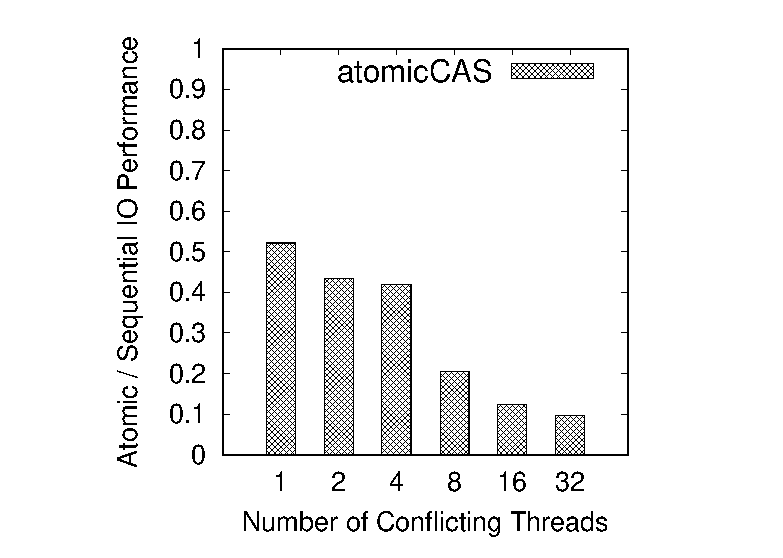
\includegraphics[width=5.3cm]{exp/atomic/atomicCAS.eps}
	\end{minipage}
	\hspace{-1em}
	\begin{minipage}{0.5\linewidth}
		\label{fig:atomicExch}
		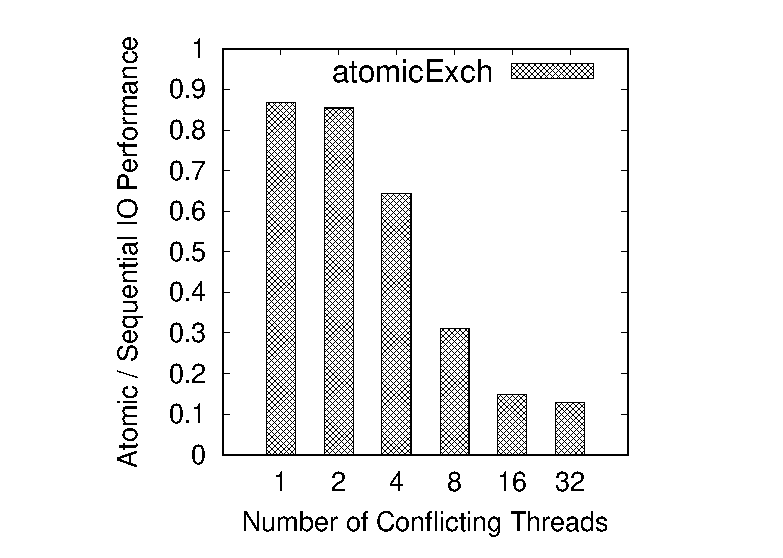
\includegraphics[width=5.3cm]{exp/atomic/atomicExch.eps}
	\end{minipage}
	\caption{The performance of atomic operations for varying number of conflicts}
	\label{fig:atomic}
\end{figure}

\begin{algorithm}[t]
	\begin{algorithmic}[1]
		\State $active \gets 1$	\label{algo:insert:active:start}
		\While{true}
		\State $l' \gets ballot(active == 1)$ \label{algo:insert:vote:start}
		\If{$l'$ is invalid}
		\State break \label{algo:insert:active:end}
		\EndIf
		\State $[(k',v'),i'] \gets broadcast(l')$ \label{algo:insert:lock:start}
		\State $loc = h^{i'}(k')$
		\If{$l' == l$}
		\State $success \gets lock(loc)$ \label{algo:insert:lock:end}
		\EndIf
		\If{$broadcast(success,l') ==$ failure}
		\State continue					\label{algo:insert:vote:end}
		\EndIf
		\State $l^* \gets ballot(loc[l].key == k' || loc[l].key ==\emptyset)$ \label{algo:insert:write:start}
		\If{$l^*$ is valid and $l' == l$}
		\State $loc[l^*].(key,val) \gets (k',v')$
		\State $unlock(loc)$
		\State $active \gets 0$;
		\State continue			\label{algo:insert:write:end}
		\EndIf
		\State $l^* \gets ballot(loc[l].key \neq \emptyset)$
		\If{$l^*$ is valid and $l' == l$}
		\State $swap(loc[l^*].(key,val),(k',v'))$
		\State $unlock(loc)$
		\State $i \gets i+1$ \label{algo:insert:loop:end}
		\EndIf
		\EndWhile
	\end{algorithmic}
	\caption{\textbf{Insert}(lane $l$, warp $wid$, kv $(k,v)$, table $i$)}\label{algo:insert}
\end{algorithm}

\vspace{1mm}\noindent\textbf{Insert.} Contention occurs when multiple \formal{insert} operations target at the same bucket. 
There are two conflicting objectives for resolving the contention. On one hand, we want to utilize the warp-centric approach to access a bucket.
On the other hand, a warp requires a mutex when updating a bucket to avoid corruption, and the locking is expensive on GPUs.  
In the literature, it is a common practice to use atomic operations for implementing a mutex under the warp-centric approach \cite{zhang2015mega}. 
In particular, we can still invoke a warp to insert a KV pair. The warp is required to acquire a lock before updating the corresponding bucket. 
The warp will keep trying to acquire the lock before successfully obtain the control. 
There are two drawbacks for this direct warp-centric approach. 
First, the conflicting warps are spinning while locking, thus wasting computing resources.
Second, although atomic operations are supported by recent GPU architectures natively, 
they become costly when the number of atomic operations issuing at the same location increases. 
In Figure~\ref{fig:atomic}, we show the profiling statistics for two atomic operations which are often used to lock and unlock a mutex: atomicCAS and atomicExch respectively. 
We compare the throughputs of the atomic operations vs. an equivalent amount of sequential device memory IOs (coalesced) and present the trend for varying the number of conflicting atomic operations. It is apparent that the atomic performance has seriously degraded for a larger number of conflicts. 
Thus, it will be expensive for the direct warp-centric approach in the contention critical cases. 
Imaging one wants to track the number of retweets posted to active twitter accounts in the current month, via storing the twitter ID and the obtained retweet counts as KV pairs. In this particular scenario, certain twitter celerities could receive thousands of retweets in a very short period. 
This triggers the same twitter ID gets updated frequently and a serious number of conflicts would happen. 

To alleviate the cost of spinning, we propose the voter-coordination scheme. 
We assign an \formal{insert} to a thread rather than using a warp to handle the operation. Before submitting a locking request and updating the corresponding bucket, the thread will participate in a vote among the threads in the same warp. 
The winner thread $l$ becomes the leader of the warp and takes control. Subsequent, the warp inspects the bucket and insert the KV for $l$ if there are spaces left, upon $l$ successfully obtaining the lock.
If $l$ fails to get the lock, the warp revotes another leader to avoid locking on the same bucket.
Compared with locking on atomic operations, the cost of warp voting is almost negligible since it is heavily optimized in the GPU architecture.  


Parallel insertion with the voter coordination scheme is presented in Algorithm~\ref{algo:insert}.
The pseudo code demonstrates how a thread (with lane $l$) from warp $wid$ inserts a KV $(k,v)$ to the $i$th hash table. 
The warp will first propose a vote among active threads and the process will terminate if all threads finish their tasks (lines~\ref{algo:insert:active:start}-\ref{algo:insert:active:end}).  
This achieves better resource utilization since no thread will be idle when one of the threads in the same warp is active.  
The leader $l'$ then broadcasts its KV pair $(k',v')$ as well as the hash table index $i'$ to the warp and tries to lock the inserting bucket (lines~\ref{algo:insert:lock:start}-\ref{algo:insert:lock:end}). 
The broadcast function ensures all threads in the warp receive the locking result and the warp revotes if $l'$ fails to obtain the lock.
Otherwise, the warp follows $l'$ and proceeds to update the bucket for $(k',v')$ with a warp-centric approach similar to \formal{find}.
Once a thread finds $k'$ or an empty space in the bucket, $l'$ will add or update with $(k',v')$ (lines~\ref{algo:insert:write:start}-\ref{algo:insert:write:end}).
Otherwise there is no space left, $l'$ swaps $(k',v')$ with a random KV in the bucket and inserts the evicted KV to hash table $i+1$ in the next round. 
In summary, each iteration of the loop presented in Algorithm~\ref{algo:insert} issues $1$ atomic operation and at most $1$ device memory read/write (lines~\ref{algo:insert:vote:start}-\ref{algo:insert:loop:end}).  

Note that we have yet covered how to choose the hash table index $i$ for each insertion (Algorithm~\ref{algo:insert}). Additional number of conflicts would happen if all threads attempting to insert to the same table. For the flow of presentation, we leave the discussion to Section~\ref{sec:dyn} since choosing the hash table is more coherent to the load balancing problem for resizing hash tables. Moreover, a careful reader would find that the insertion process could lead to multiple appearances of the same key in different hash tables. To fill this gap, one can attach a timestamp to the insertion batch.
Hence, the \formal{find} operation is required to scan all $d$ buckets of the same key and extracts the one with the latest timestamp.

\begin{figure}[t]
	\centering
	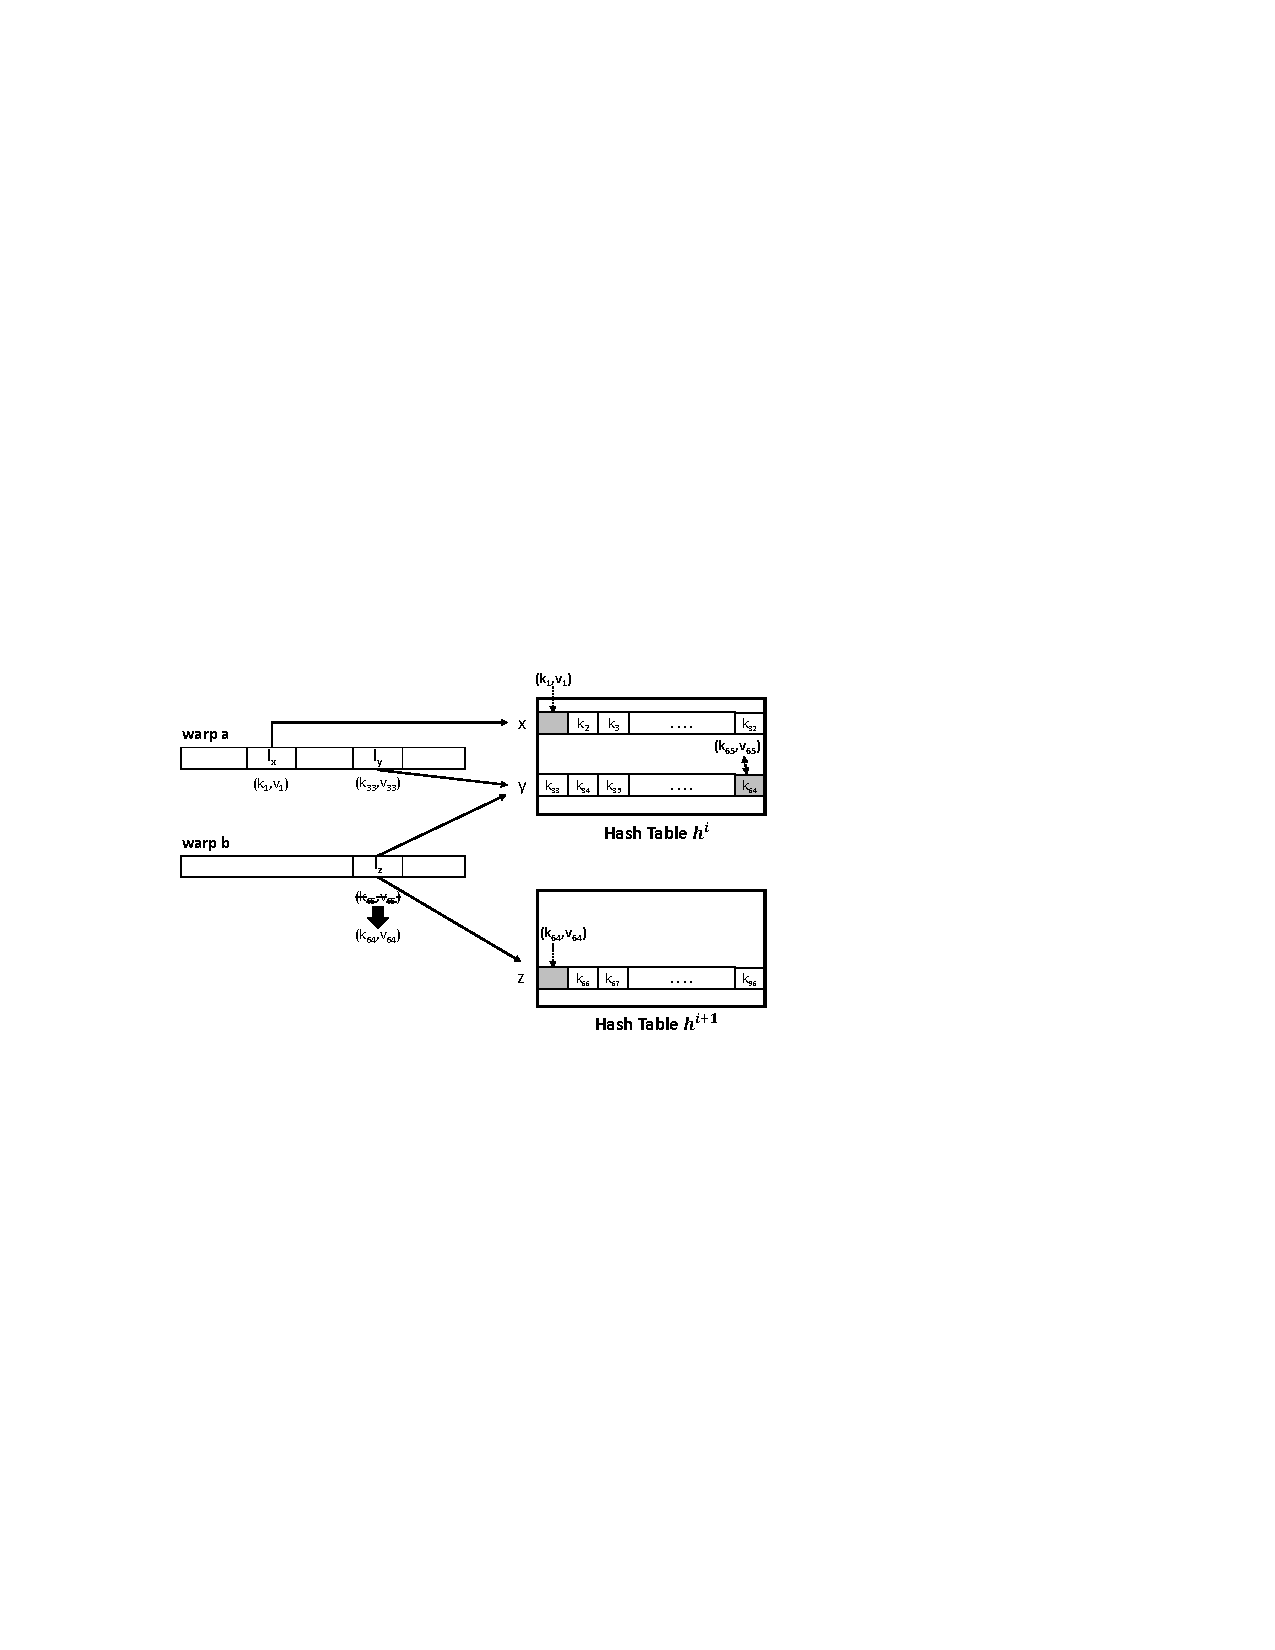
\includegraphics[width=0.45\textwidth]{fig/Voter.pdf}
	\caption{Example for parallel insertions}
	\label{fig:voter}
\end{figure}

We give the following example to demonstrate the parallel insertion process.
\begin{example}
	In Figure~\ref{fig:voter}, we visualize the scenario for three threads: $l_x$, $l_y$, $l_z$ from two warps, inserting KV pairs $(k_1,v_1)$,$(k_{33},v_{33})$,$(k_{65},v_{65})$ independently. 
	Suppose $l_y$ and $l_z$ become the leaders of warp $a$ and $b$ respectively. Both threads will compete for the bucket $y$ and $l_z$ wins the battle. 
	$l_z$ will then leads warp $b$ to inspect the bucket and evict $(k_{64},v_{64})$ by replacing with $(k_{65},v_{65})$. 
	In the meanwhile, $l_y$ does not lock on bucket $y$ and joins the new leader $l_x$ voted in warp $a$. 
	$l_x$ locks bucket $x$ and inserts $(k_1,v_1)$ in place. Subsequently, $l_y$ may get back the control of warp $a$ and update $k_{33}$ with $(k_{33},v_{33})$ at bucket $y$. In parallel, $l_z$ locks bucket $z$ and inserts the evicted KV $(k_{64},v_{64})$ into the empty space. 
\end{example}

\vspace{1mm}\noindent\textbf{Delete.} The \formal{delete} operation, in contrast to \formal{insert}, does not require locking with a warp-centric approach. 
Similar to \formal{find}, we assign a warp to process a key $k$ on deletion. The warp iterates through the buckets among all $d$ hash tables that could possibly contain $k$. Each thread lane in the warp is responsible for inspecting one position in a bucket independently, and only erase the key if $k$ is found, 
thus causes no contention.

%\begin{algorithm}[t]
%	\begin{algorithmic}[1]
%		\For{$i=1,\ldots,d$}
%			\State $loc \gets h^i(k)$
%			\State $found \gets (loc[l].key == k)$
%			\If{$found$}
%				\State $loc[l].key \gets \emptyset$
%			\EndIf
%		\EndFor
%	\end{algorithmic}
%	\caption{\textbf{Delete}(lane $l$, warp $wid$, key $k$)}\label{algo:delete}
%\end{algorithm}


\vspace{1mm}\noindent\textbf{Complexity.}
Since a \formal{find}, \formal{insert} and \formal{delete} operation is independently executed by a thread. 
The analysis of a single thread complexity is the same as the sequential version of cuckoo hashing \cite{pagh2004cuckoo}: $O(1)$ worst case complexity for \formal{find} and \formal{delete}, $O(1)$ expected time for \formal{insert} for the case of 2 hash tables. 
It has been pointed out that analyzing the theoretical upper bound complexity of insertion in $d \geq 3$ hash tables is very difficult \cite{alcantara2009real}.  
Nevertheless, empirical results have shown that increasing the number of tables leads to better insertion performance, see our experiments in Section~\ref{sec:exp}.
Thus, we assume the complexity for inserting to $d$ hash tables is the same as that of $2$ has tables, as long as $d$ keeps constant.  

We then analyze the number of possible thread conflicts. Assuming we launch $m$ threads in parallel, each of them is assigned to an unique key, and the total number of unique buckets is $H=\sum_{i=1}^d|h^i|$. For \formal{find} and \formal{delete}, there is no conflict at all. 
For \formal{insert}, computing the expected number of conflicting buckets resembles the \emph{balls and bins} problem \cite{raab1998balls}, which is $O(\binom{m}{2}/H)$. 
Given GPUs have a large number of threads, there could be a significant amount of conflicts. Thus, we propose the voter coordination scheme to reduce the cost of spinning on locks. Note that the analysis is done for the cases where the key to update is unique. More conflicts could occur in reality when the same key is updated in parallel. 
\section{experimental evaluation}\label{sec:exp}
In this section, we conduct extensive experiments by comparing the proposed hash table designs with several state-of-the-art approaches for GPU-based hash tables. 
We will introduce the experimental setup and the discuss the results. 

\subsection{Experiment Setup}\label{sec:exp:setup}

\vspace{1mm}\noindent\textbf{Baselines.} We compare the proposed approach in this paper with several state-of-the-art hash table implementations on GPUs and CPUs. 
\begin{itemize}
	\item \cudpp is a popular CUDA primitive library which contains the cuckoo hash table implementation published in~\cite{alcantara2009real}. 
	\cudpp employs four hashing function and each hash value stores only one KV pair with 64 bits size (32 bits for key and 32 bits for value). 
	\cudpp only supports \formal{insert} and \formal{find} operations. 
	\item \megakv is a state-of-the-art approach for GPU-based key value store published in~\cite{zhang2015mega}. It employs a cuckoo hash with two hash functions.
	\megakv also allocates a bucket for each hash value. However, it does not lock a bucket when performing update. Instead, it uses intra-block synchronization to resolve race condition. 
	\item \linear is a GPU-based hash table which uses linear open addressing to resolve conflicts \cite{hong2010mapcg}. 
	\item \google is an efficient CPU-based hash table implementation\footnote{https://github.com/sparsehash/sparsehash-c11/}. We choose the \emph{dense\_hash\_map} implementation since it provides the best efficiency.
	\item \voter is the approach proposed in this paper.
\end{itemize}
We adopt the original implementations of \cudpp and \google from their corresponding inventors. 
For \megakv, we note that its intra-block synchronization could lead to inconsistency issue as well as a large number of insertion failures, especially when the filled factor is high.  
Thus, we revise its code by replacing the intra-block synchronization with atomicExch to resolve the race condition. The adoption of atomicExch preserves the design principle of \megakv for \emph{not} locking the entire bucket for updates. Moreover, it leads to less insertion failures and similar performance against its original implementation. 
For \linear, we implement the CUDA version of the algorithm proposed in \cite{hong2010mapcg}.

Note that we do not compare with the dynamic GPU hash approach proposed in \cite{ashkiani2018dynamic} for two major reasons. First, we cannot obtain the original implementation from its authors. Second, the approach devises a dedicated memory allocator other than cudaMalloc. A dedicated allocator will improve the performance but add complexity the system. Additionally, it needs to occupy a large memory in advance and is not transparent to other GPU applications.
In contrast, our proposed approach only use native allocator supported. 
We do not compare with \cite{breslow2016horton} since it only improves \megakv marginally using a more costly insertion process.

\begin{table}[t]
	\caption{The datasets used in the experiments.}
	\label{table:exp_data_sets}
	\centering
	\begin{tabular}{|c|c|c|c|}
		\hline
		Datasets & KV pairs & Unique keys & Max Duplicates \\ \hline
		\dstwitter &50,876,784 & 44,523,684&\\ \hline
		\dsreddit & 48,104,875 & 41,466,682 & \\ \hline
		\dstpch &50,000,000 & 45,159,880&\\ \hline
		\dsali &10,000,000 & 4,583,941&\\ \hline
		\dsrandom & 100,000,000& 100,000,000& 1 \\ \hline
	\end{tabular}
\end{table}

\vspace{1mm}\noindent\textbf{Datasets.} We evaluate all compared approaches using several real world and synthetic datasets described as follows:
\begin{itemize}
	\item \dstwitter: Twitter is an online social network where users perform actions include \emph{tweet}, \emph{retweet}, \emph{quote} and \emph{reply}.
	We crawl these actions for one week via Twitter stream API\footnote{https://dev.twitter.com/streaming/overview} on trending topics US president election, 2016 NBA finals and Euro 2016. The dataset contains 50,876,784 KV pairs.
	\item \dsreddit: Reddit is an online forum where users perform actions include \emph{post} and \emph{comment}. We collect all Reddit \emph{comment} actions in May 2015 from \emph{kaggle}\footnote{https://www.kaggle.com.reddit/reddit-comments-may-2015} and query the Reddit API for the \emph{post} actions the same period. The dataset contains 48,104,875 actions as KV pairs. 
 	\item \dstpch: Lineitem is a synthetic table generated by the TPC-H benchmark\footnote{https://github.com/electrum/tpch-dbgen}. We generate  100,000,000 rows of the lineitem table and combine the \emph{orderkey},\emph{linenumber} and \emph{partkey} column as keys. 
	\item \dsrandom: Random is a synthetic dataset generated from a normal distribution. We have deduplicated the data and generate 100,000,000 KV pairs.  
	\item \dsali: Databank is a PB-scale data warehouse that stores user behavior data in past one year of Alibaba's economic entity. Due to confidentially, we sample 10,000,000 transactions and the dataset contains 4,583,941 unique data ids as keys.
\end{itemize}
The summary of the datasets can be found in Table~\ref{table:exp_data_sets}.
Since all GPU approaches (except for \voter) only supports 32 bit key and 32 bit value, we hash longer keys to 32 bits and truncate all values to 32 bits across all datasets. 


\begin{table}
	\centering
	\caption{Parameters in the experiments}
	\label{tbl:parameters}
	\begin{tabular}{|c|c|c|}
		\hline
		\textbf{Parameter} & \textbf{Settings} & \textbf{Default} \\ \hline
		$\alpha$ & 25\%, 30\%, 35\%, 40\%, 45\% & 40\% \\ \hline
		$\beta$  & 75\%, 80\%, 85\%, 90\%, 95\% & 90\% \\ \hline
		$r$ & 0.1, 0.2, 0.3, 0.4, 0.5 & 0.4 \\ \hline
	\end{tabular}
\end{table}

\vspace{1mm}\noindent\textbf{Static Hashing Comparison (Section~\ref{sec:exp:static}).}
Under the static setting, we evaluate \formal{insert} and \formal{find} performance among all compared approaches. 
In particular, we insert all KV pairs from the datasets followed by issuing 1 million random search queries. 

\vspace{1mm}\noindent\textbf{Dynamic Hashing Comparison (Section~\ref{sec:exp:dynamic}).}
Under the dynamic setting, we generate the workloads by batching the hash table operations. 
We partition the datasets into batches of $1$ million insertions. 
For each batch, we augment $1$ million \formal{find} operations and $1 \cdot r$ million \formal{delete} operations,
where $r$ is a parameter to balance insertions and deletions.
After we exhaust all the batches obtained from the datasets, we rerun these batches by swapping the \formal{insert} and \formal{delete} operations in any batch. 
We evaluate the performance of all compared approaches except \cudpp as it does not support deletions. 
Since all approaches other than \voter are static hash tables, we double/half the memory usage followed by rehashing all KV pairs as their resizing strategy, if the corresponding filled factor falls out of the specified range. 
Moreover, if an insertion failure is found for a compared approach, we trigger its resizing strategy.


\vspace{1mm}\noindent\textbf{Parameters.}
We vary the parameters when comparing \voter with the baselines.
$\alpha$ is the lower bound on the filled factor $\theta$ for all compared approaches,
whereas $\beta$ is the respective upper bound.
$r$ is the ratio of insertions over deletions in a processing batch. 
The settings of the aforementioned parameters could be found in Table~\ref{tbl:parameters}.

\vspace{1mm}\noindent\textbf{Experiment Environment.}
We conduct the experiments on an Intel Xeon E5-2620 Server equipped with NVIDIA GeForce GTX 1080.The GTX 1080 is built on Pascal architecture with 20 SMs and 128 SPs per SM. The GTX 1080 has 8 GB of GDDR5 memory. Evaluations are performed using CUDA 8.0 on Ubuntu 16.04.3. The optimization level (-O3) is applied for compiling all programs.


\subsection{Tunning Parameters}

A key parameter that affects the performance of \voter is the number of hash table chosen. For the static scenario, we present the throughput performance of \formal{insert} and \formal{find} for varying number of hash tables in Figure~\ref{fig:vary-table}, while fixing the memory space of the entire structure to ensure the default filled factor. 
The throughput of \formal{insert} increases with more hash tables, since there are more alternative locations for inserting a KV pair. However, the marginal improvement drops for a larger number of hash tables. The throughput of \formal{find} falls with more hash tables as additional locations need to be scanned to locate a KV pair. Thus, one can tradeoff the performance between \formal{insert} and \formal{find} operations by varying the number of tables. In this paper, we choose three hash tables as our default implementation as it provides the best balance. 


\begin{figure}[t!]
\begin{minipage}{0.48\linewidth}\centering
	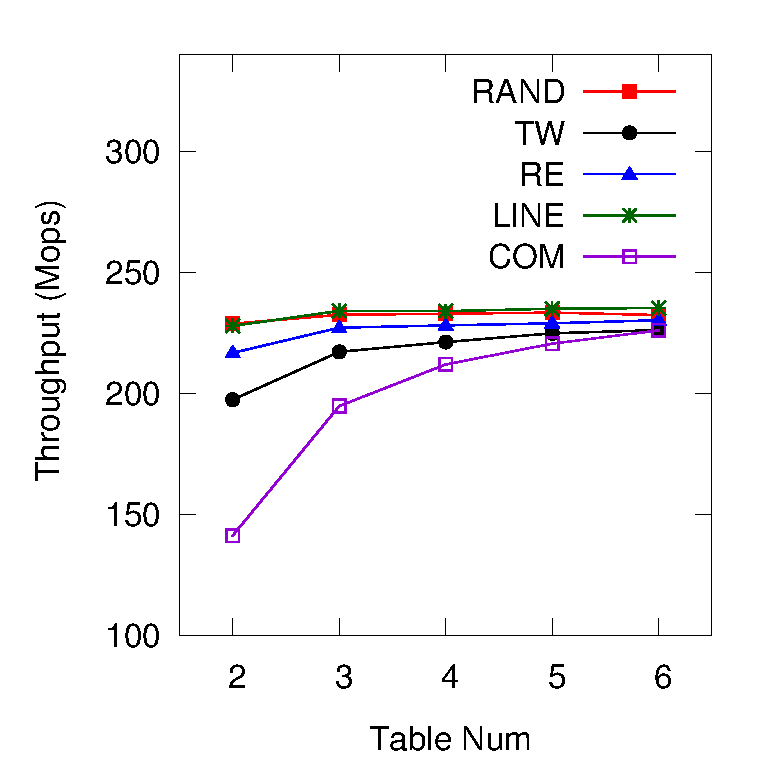
\includegraphics[width=\linewidth]{pic/tunning/tunning-insert.eps}
	\centerline{\formal{insert}}
	\end{minipage}
	\hfill
	\begin{minipage}{0.48\linewidth}\centering
	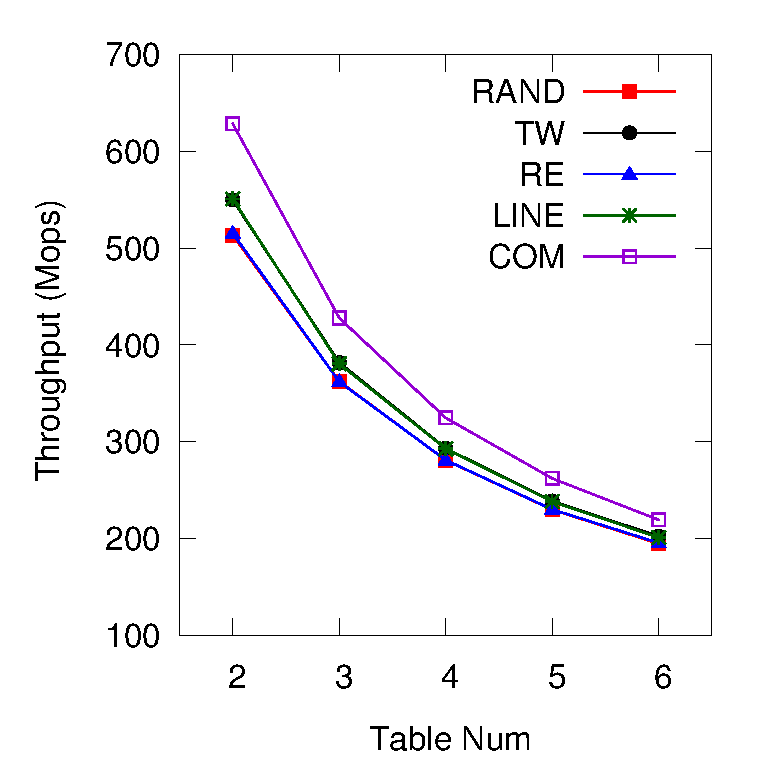
\includegraphics[width=\linewidth]{pic/tunning/tunning-search.eps}
	\centerline{\formal{find}}
	\end{minipage}
	\caption{Throughput of \voter when varying the number of hash tables.}
	\label{fig:vary-table}
\end{figure}

\subsection{Static Hashing Comparison}\label{sec:exp:static}

\vspace{1mm}\noindent\textbf{Throughput Analysis.} We present the throughput of all compared approaches in Figure~\ref{fig:static} when varying the filled factor. 
First of all, GPU-based approaches are orders of magnitude faster than \google (2  million ops for \formal{insert} and 6 million ops for \formal{find} on average), which validates the motivation of designing hash tables on GPUs. 
Among GPU hash tables, \megakv delivers the best performance across all datasets except for \dsali. Nevertheless, for \formal{insert}, the drawback of \megakv is that it fails to insert some of the KV pairs. Tables~\ref{tab:fail:tw}-\ref{tab:fail:com} present the percentages of insertion failure for varying filled factor across all datasets. \megakv has up to 2.5\% failure rate for the default filled factor, which is the highest among all approaches. 
Our proposed \voter has the lowest failure rate and achieve the 2nd best performance behind \megakv. We note that \cudpp obtains a significant advantage over all approaches in the \dsali dataset. This is because \cudpp will immediately terminate its GPU kernel once it finds some KV pairs cannot be inserted after a number of lookups. This explains why \cudpp has a superior performance since it early terminates on \dsali due to failed insertions (Table~\ref{tab:fail:com}). For \formal{find}, \megakv achieves the best performance as it only has two hash functions. This explains why \voter is slower since we use three hash tables and additional IO lookups are required for each \formal{find}. Both \megakv and \voter are faster than \cudpp and \linear since they employs the bucket mechanism for storing multiple KV pairs contiguously under the same hash value, which exhibits better coalesced memory access.  

\begin{figure}[t!]
	\begin{minipage}{0.48\linewidth}\centering
		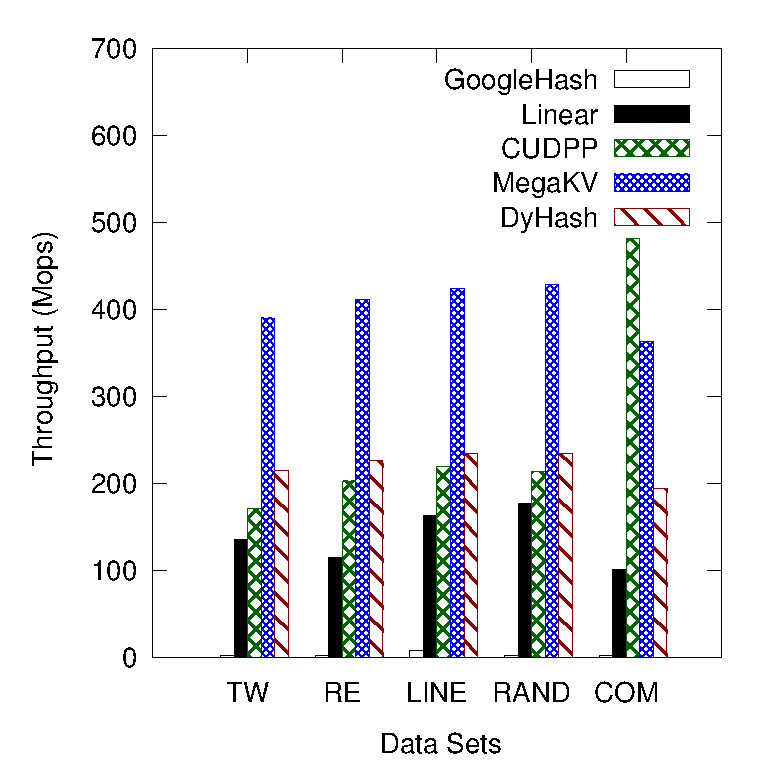
\includegraphics[width=\linewidth]{pic/static/static_insert.eps}
		\centerline{\formal{insert}}
	\end{minipage}
	\hfill
	\begin{minipage}{0.48\linewidth}\centering
		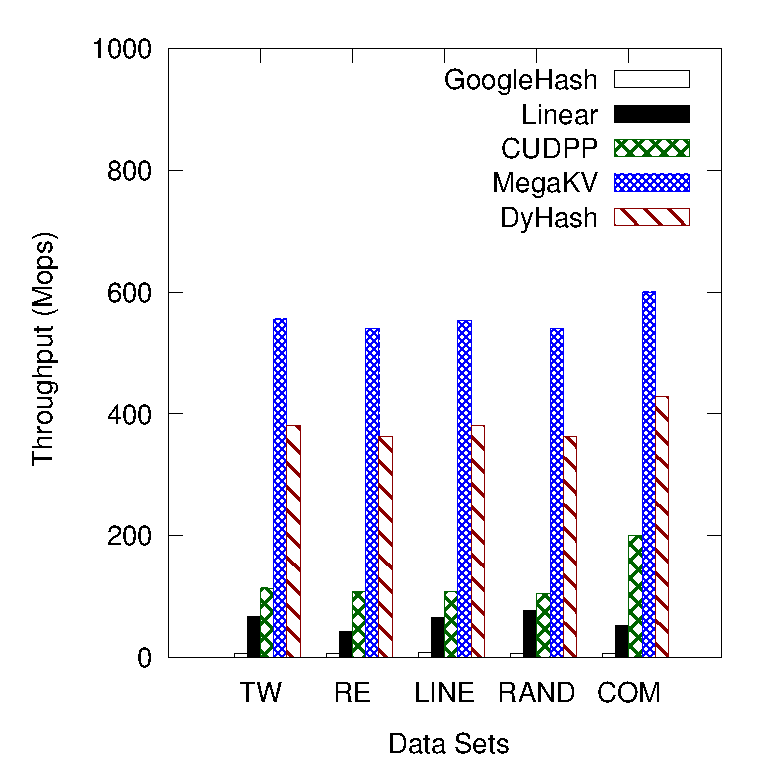
\includegraphics[width=\linewidth]{pic/static/static_search.eps}
		\centerline{\formal{find}}
	\end{minipage}
	\caption{Throughput of all compared approaches under the static setting.}
	\label{fig:static}
\end{figure}
\begin{figure*}[t]
	\begin{minipage}{0.3\linewidth}\centering
		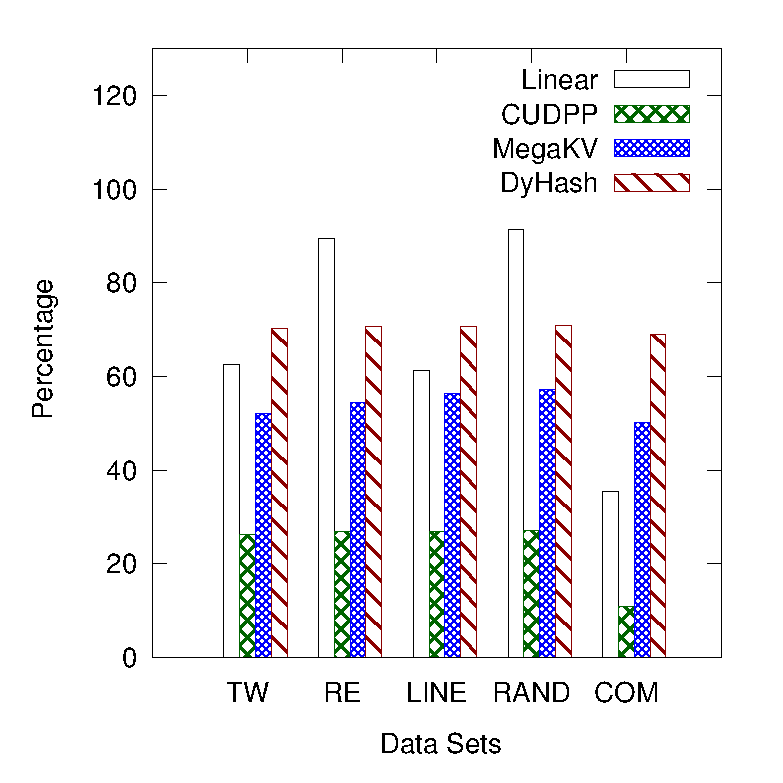
\includegraphics[width=\linewidth]{pic/static-profi/warp.eps}
		\centerline{Warp Efficiency}
	\end{minipage}
	\hfill
	\begin{minipage}{0.3\linewidth}\centering
		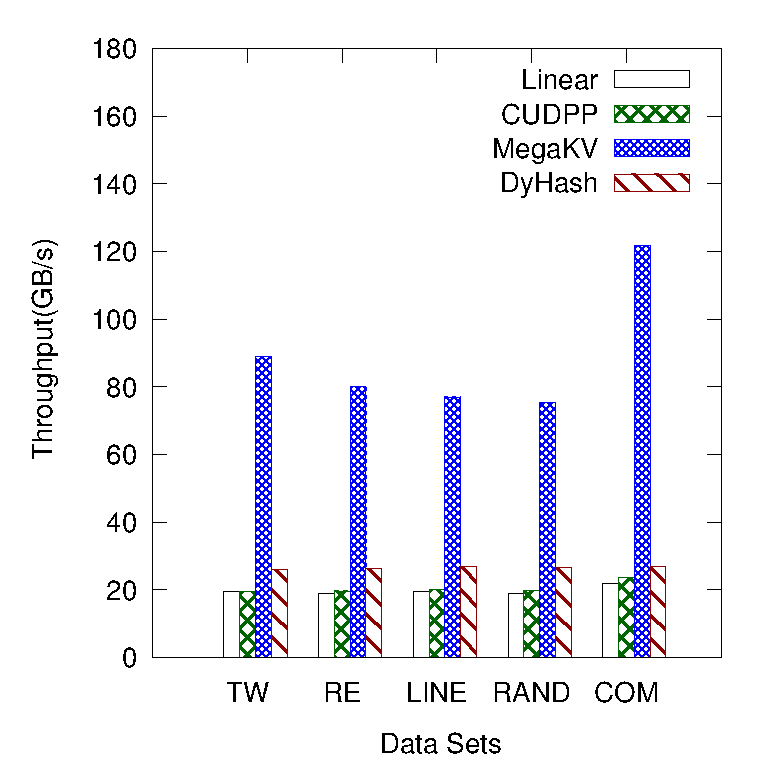
\includegraphics[width=\linewidth]{pic/static-profi/L2-read.eps}
		\centerline{Cache Utilization}
	\end{minipage}
	\hfill
	\begin{minipage}{0.3\linewidth}\centering
		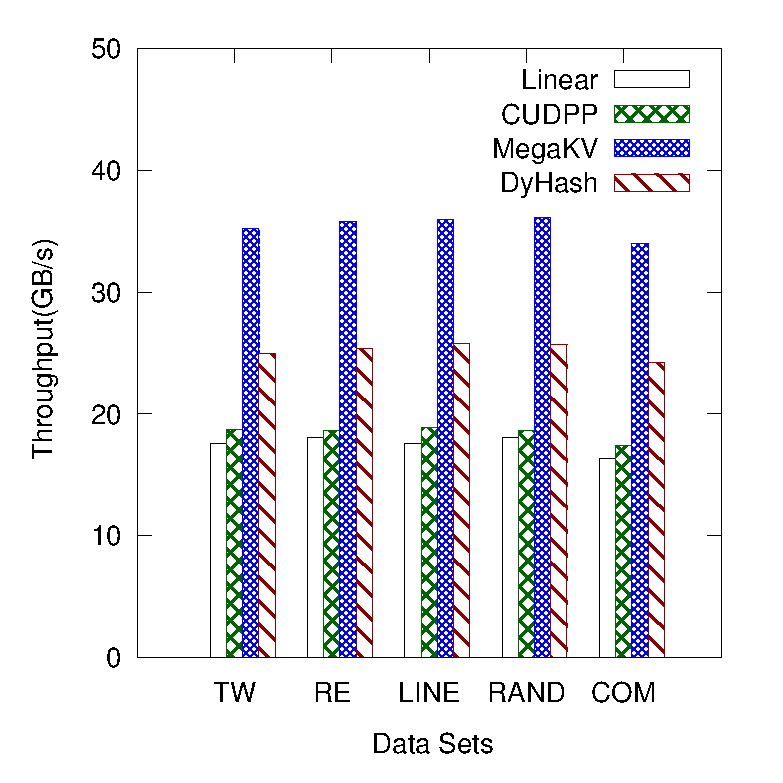
\includegraphics[width=\linewidth]{pic/static-profi/memory-read.eps}
		\centerline{Memory Bandwidth Utilization}
	\end{minipage}
	\caption{GPU profiling results for static hashing comparison.}
	\label{fig:static:profile}
\end{figure*}

For interested readers, please find the throughput results for varying the filled factor across all datasets in the appendix (Figure~\ref{fig:static:all:insert} and~\ref{fig:static:all:search}). 



\vspace{1mm}\noindent\textbf{GPU Profiling.} To further study the behavior of the approaches, we present three types of profiling results for all \formal{insert} GPU kernels in Figure~\ref{fig:static:profile}.
For \emph{warp efficiency}, \voter maintains a stable rate at around 70\%, which is significantly higher than the other two cuckoo hash approaches: \megakv and \cudpp.  
We attribute this phenomenon to the voter mechanism proposed in Section~\ref{sec:vot:con}, which yields better overall load balancing. 
\linear could achieve higher warp efficiency than \voter, but is very volatile across different datasets. This is because each \formal{insert} in \linear may require scanning varying number of hash values for distinct data distributions. 
For example, in the \dsali dataset, its warp efficiency drops below 40\% since \dsali contains more duplicated keys than other datasets. 

Looking at \emph{cache} and \emph{memory bandwidth} profiling results, \megakv and \voter achieve better utilization as they employ the bucket mechanism.
As \voter always needs to use atomicCAS to lock a bucket before accessing it, its utilization is inferior than that of \megakv due to the additional IO when inserting a KV pair to a bucket. In addition, atomicCAS is less efficient than atomicExch as it involves more workloads per operation (see Table~\ref{fig:atomic}). Nevertheless, implementations based on atomicExch only supports KV pair with 64 bits, whereas adopting atomicCAS in \voter can support arbitrary length as we lock the bucket for exclusive update.
It is also noted that, even though \megakv has great cache utilization due to the use of atomicExch accessing buckets directly, the overall performance is eventually bounded by device memory IOs. 

In summary, under the static environment, \voter achieves competitive efficiency against the compared GPU baselines. Moreover, although \voter does not deliver the best performance over existing approaches, it has zero insertion failure rate and supports more general hash tables.





\subsection{Dynamic Hashing Comparison}\label{sec:exp:dynamic}

\vspace{1mm}\noindent\textbf{Varying the filled factor lower bound $\alpha$.}
We vary the lower bound of the filled factor and report the results in Figure~\ref{fig:vary-alpha-time}. 
The performance is measured by the total running time for processing all batches described in Section~\ref{sec:exp:setup}. Furthermore, we indicate the time taken for all components involved in the processing: \formal{insert}, \formal{find}, \formal{delete} and \formal{resize}. Apparently, the resizing strategy adopted by \linear and \megakv incur significant overhead. Such an overhead grows dramatically for a higher $\alpha$ since more downsizing is required. It is noted that the impact of resizing is the more significant for \megakv than \linear. We interpret the phenomenon as the following.
\megakv has a higher insertion failure rate than that of \linear (see Table~\ref{tab:fail:tw}-\ref{tab:fail:com}). Thus \megakv triggers more upsizing operations leading to a lower filled ratio when resized. As each processing batch contains deletions, \megakv is prone to downsizing when the filled factor falls below $\alpha$ after deletions materialize.
The overhead of repeated upsizing and downsizing severely degrades the performance of \megakv, for the major reason of maintaining the filled factor above $\alpha$. 
The only exception is where $\alpha$ is very small (i.e., $\alpha=0.25$) and \megakv does not need to perform downsize regularly. However, small $\alpha$ means the hash table is mostly empty and thus wastes GPU memory resources.
In contrast, \voter achieves significant speedups over \linear and \megakv (up to \xxx and \xxx faster respectively under the default setting). 
\voter can support even larger $\alpha$ (i.e., $\beta\cdot\frac{d}{d+1}$) but we omit the results since the baselines cannot deliver reasonable performance beyond $\alpha > 0.5$.
There are two reasons behind the results. First, \voter has near-zero failure rate and thus avoids unnecessary upsizing and downsizing operations. Second, \voter employs the resizing strategy (proposed in Section~\ref{sec:dyn}) by only relocating the entries in one subtable efficiently. 
Compared with time taken by \formal{insert}, \formal{delete} and \formal{find}, the cost of \formal{resize} for \voter is almost negligible as shown by the results. 

\begin{figure*}[t]
	\begin{minipage}{0.19\linewidth}\centering
		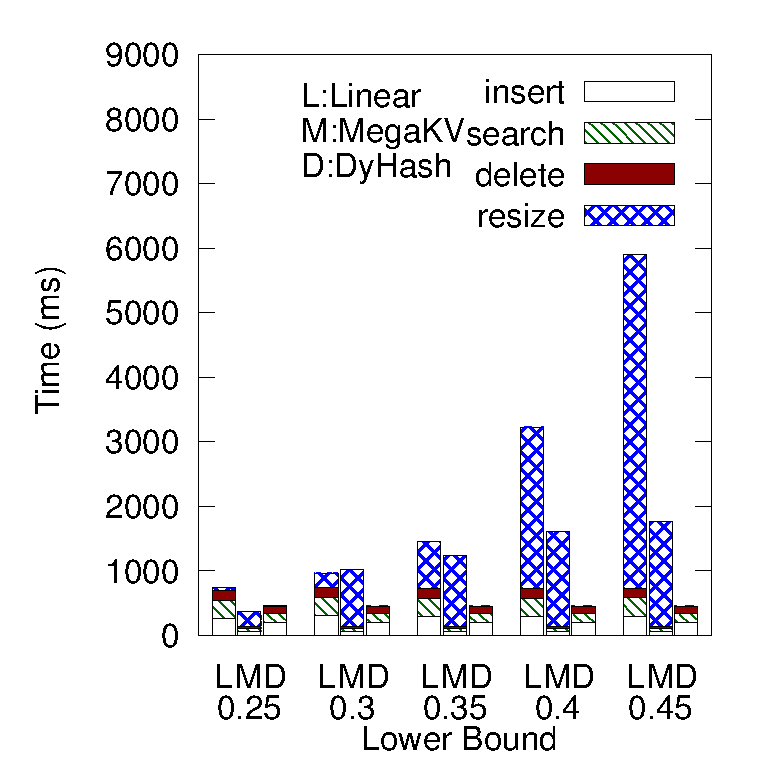
\includegraphics[width=\linewidth]{pic/dynamic/twitter/diff_lower.eps}
		\centerline{\dstwitter}
	\end{minipage}
	\begin{minipage}{0.19\linewidth}\centering
		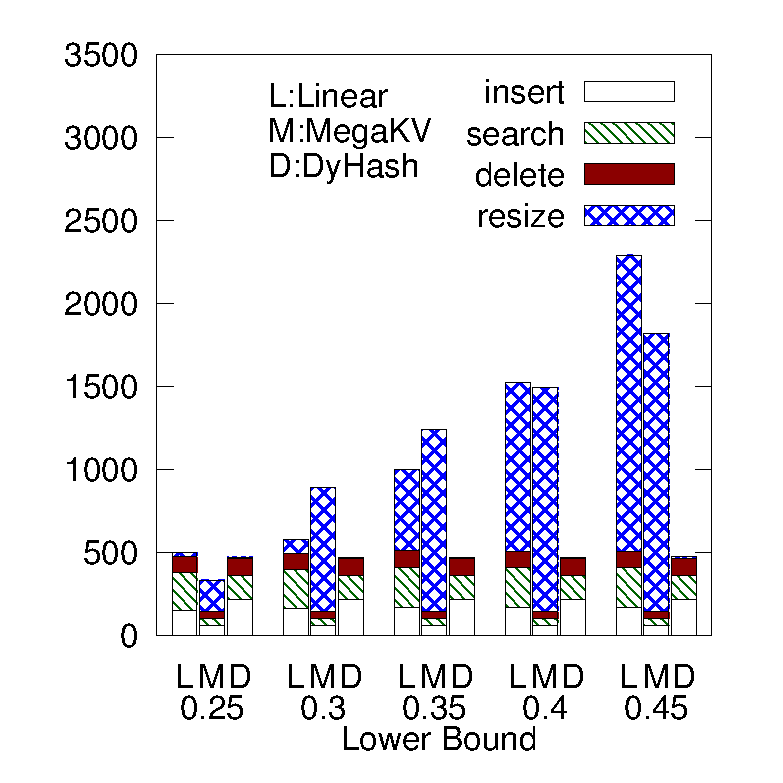
\includegraphics[width=\linewidth]{pic/dynamic/reddit/diff_lower.eps}
		\centerline{\dsreddit}
	\end{minipage}
	\begin{minipage}{0.19\linewidth}\centering
		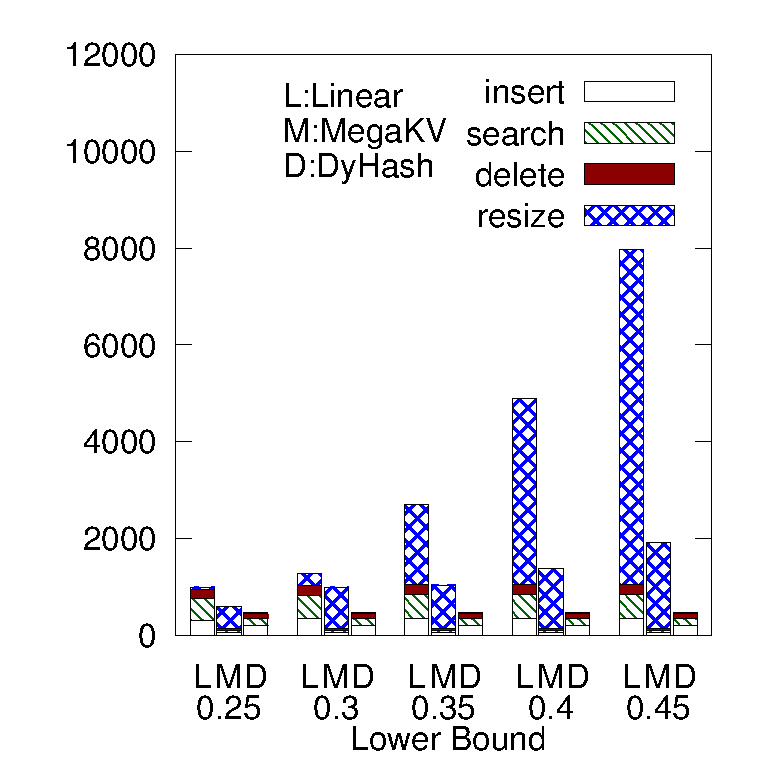
\includegraphics[width=\linewidth]{pic/dynamic/tpch/diff_lower.eps}
		\centerline{\dstpch}
	\end{minipage}
	\begin{minipage}{0.19\linewidth}\centering
		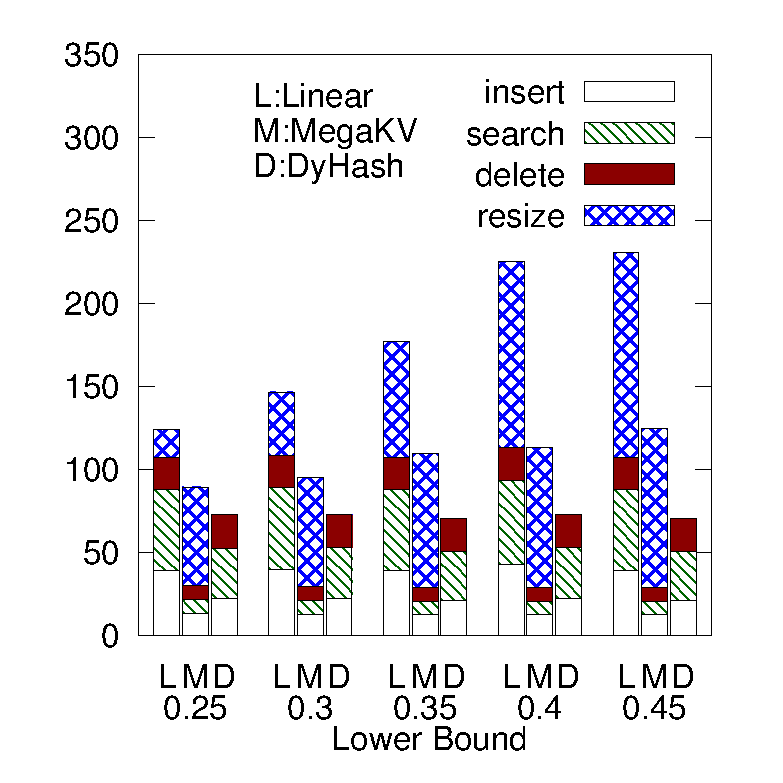
\includegraphics[width=\linewidth]{pic/dynamic/ali/diff_lower.eps}
		\centerline{\dsali}
	\end{minipage}
	\begin{minipage}{0.19\linewidth}\centering
		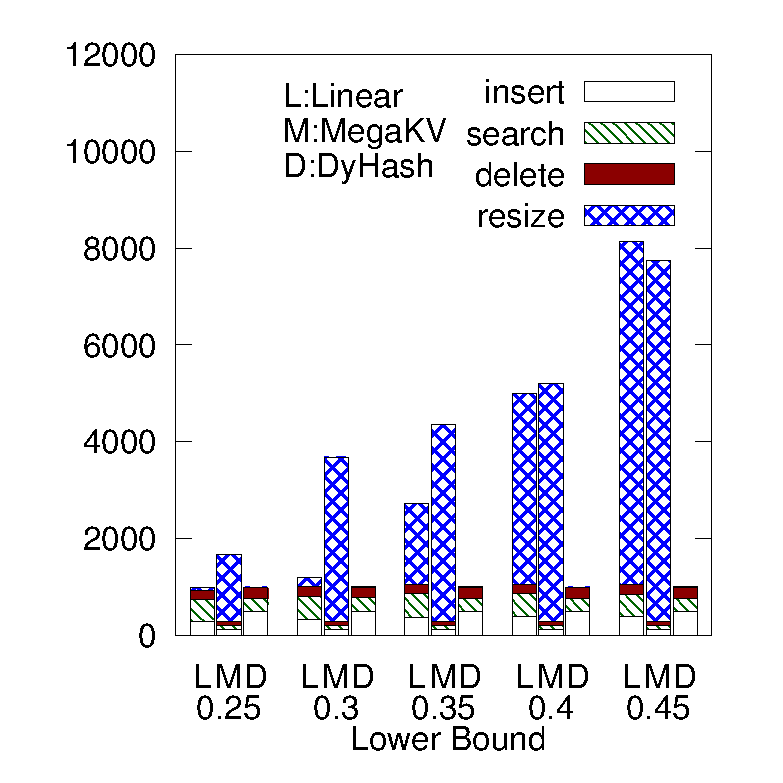
\includegraphics[width=\linewidth]{pic/dynamic/random/diff_lower.eps}
		\centerline{\dsrandom}
	\end{minipage}
	\caption{Run time for varying $\alpha$.}
	\label{fig:vary-alpha-time}
\end{figure*}

\begin{table*}{t}\centering
	\begin{minipage}{0.45\linewidth}\centering
		\caption{The failure of TW (Percentages).}
		\begin{tabular}{|c|c|c|c|c|c|}
			\hline
			& 0.75 & 0.8 & 0.85 & 0.9 & 0.95\\ \hline
			Linear &0.0 & 0.0 &4.6e-5  & 1.1e-3 & 3.9e-1 \\ \hline
			CUDPP & 0.0 & 0.0 &0.0  & 0.0 & 0.0 \\ \hline
			MegaKV & 3.4e-1 & 5.6e-1 &8.9e-1 & 1.4 & 2.0 \\ \hline
			DyHash &0.0 & 0.0 &0.0  & 0.0 & 0.0 \\ \hline
		\end{tabular}
		\label{tab:fail:tw}
	\end{minipage}
	\begin{minipage}{0.45\linewidth}\centering
		\caption{The failure of RE (Percentages).}
		\begin{tabular}{|c|c|c|c|c|c|}
			\hline
			& 0.75 & 0.8 & 0.85 & 0.9 & 0.95\\ \hline
			Linear &5.6e-3 & 1.5e-2 &1.8e-2  & 2.0e-2 & 2.0 \\ \hline
			CUDPP & 0.0 & 0.0 &0.0  & 0.0 & 0.0 \\ \hline
			MegaKV &5.1e-1 & 8.8e-1 &1.5  & 2.3 & 3.5 \\ \hline
			DyHash &0.0 & 0.0 &0.0  & 1.0e-6 & 1.0e-6 \\ \hline
		\end{tabular}
		\label{tab:fail:re}
	\end{minipage}
	\begin{minipage}{0.45\linewidth}\centering
		\caption{The failure of LINE (Percentages).}
		\begin{tabular}{|c|c|c|c|c|c|}
			\hline
			& 0.75 & 0.8 & 0.85 & 0.9 & 0.95\\ \hline
			Linear &0.0 & 0.0 &1.1e-4  & 1.8e-3 & 3.9e-1 \\ \hline
			CUDPP & 0.0 & 0.0 &0.0  & 0.0 & 0.0 \\ \hline
			MegaKV &4.6e-1 & 8.4e-1 &1.5  & 2.5 & 3.9 \\ \hline
			DyHash &0.0 & 0.0 &0.0  & 2.0e-6 & 4.0e-6 \\ \hline
		\end{tabular}
		\label{tab:fail:line}
	\end{minipage}
	\begin{minipage}{0.45\linewidth}\centering
		\caption{The failure of RAND (Percentages).}
		\begin{tabular}{|c|c|c|c|c|c|}
			\hline
			& 0.75 & 0.8 & 0.85 & 0.9 & 0.95\\ \hline
			Linear &8.4e-5 & 4.1e-4 &5.7e-4  & 8.7e-4 & 2.0 \\ \hline
			CUDPP & 0.0 & 0.0 &0.0  & 0.0 & 0.0 \\ \hline
			MegaKV &4.2e-1 & 7.9e-1 &1.4  & 2.4 & 3.9 \\ \hline
			DyHash &0.0 & 0.0 &0.0  & 0.0 & 0.0 \\ \hline
		\end{tabular}
		\label{tab:fail:rand}
	\end{minipage}
	\begin{minipage}{0.45\linewidth}\centering
		\caption{The failure of COM (Percentages).}
		\begin{tabular}{|c|c|c|c|c|c|}
			\hline
			& 0.75 & 0.8 & 0.85 & 0.9 & 0.95\\ \hline
			Linear &0.0 & 0.0 &2.0e-5  & 6.5e-4 & 2.5e-2 \\ \hline
			CUDPP & 0.0 & 0.0 &0.0  & 0.0 & 0.0 \\ \hline
			MegaKV &6.1e-2 & 8.0e-1 &1.0  & 1.3 & 1.5 \\ \hline
			DyHash &0.0 & 0.0 &0.0  & 0.0 & 7.1e-4 \\ \hline
		\end{tabular}
		\label{tab:fail:com}
	\end{minipage}
\end{table*}

\begin{figure*}[t]
	\begin{minipage}{0.19\linewidth}\centering
		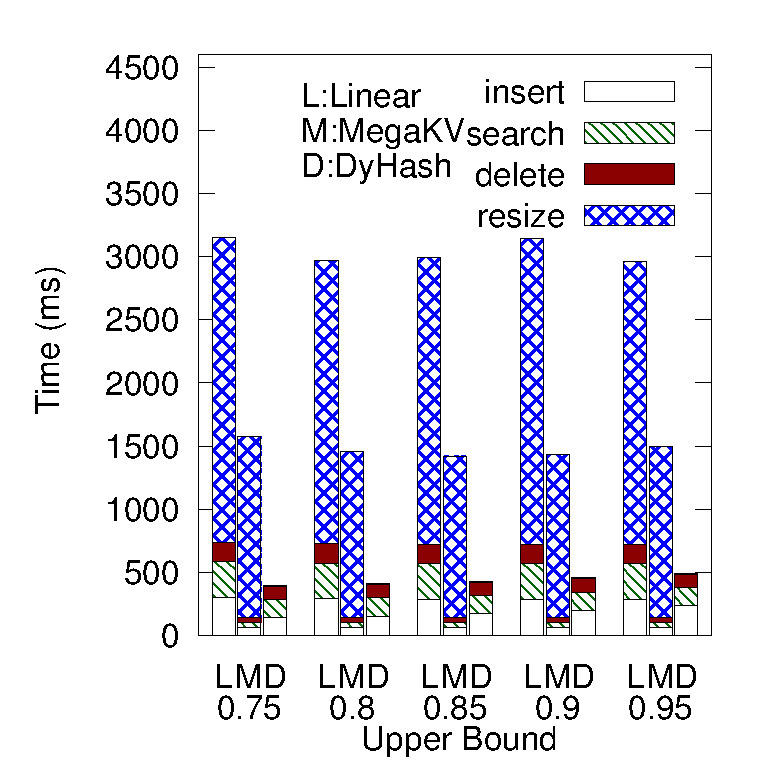
\includegraphics[width=\linewidth]{pic/dynamic/twitter/diff_upper.eps}
		\centerline{\dstwitter}
	\end{minipage}
	\begin{minipage}{0.19\linewidth}\centering
		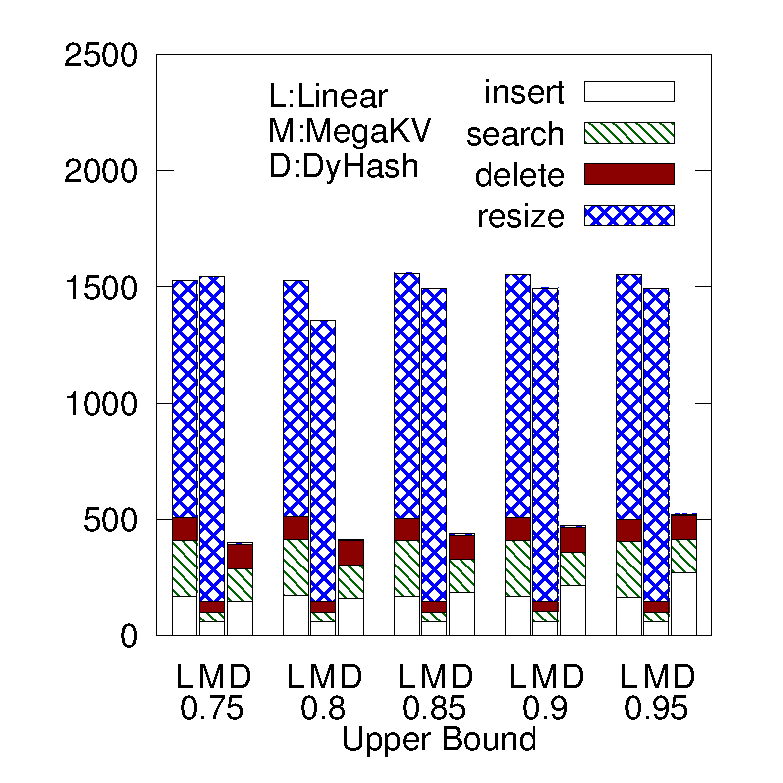
\includegraphics[width=\linewidth]{pic/dynamic/reddit/diff_upper.eps}
		\centerline{\dsreddit}
	\end{minipage}
	\begin{minipage}{0.19\linewidth}\centering
		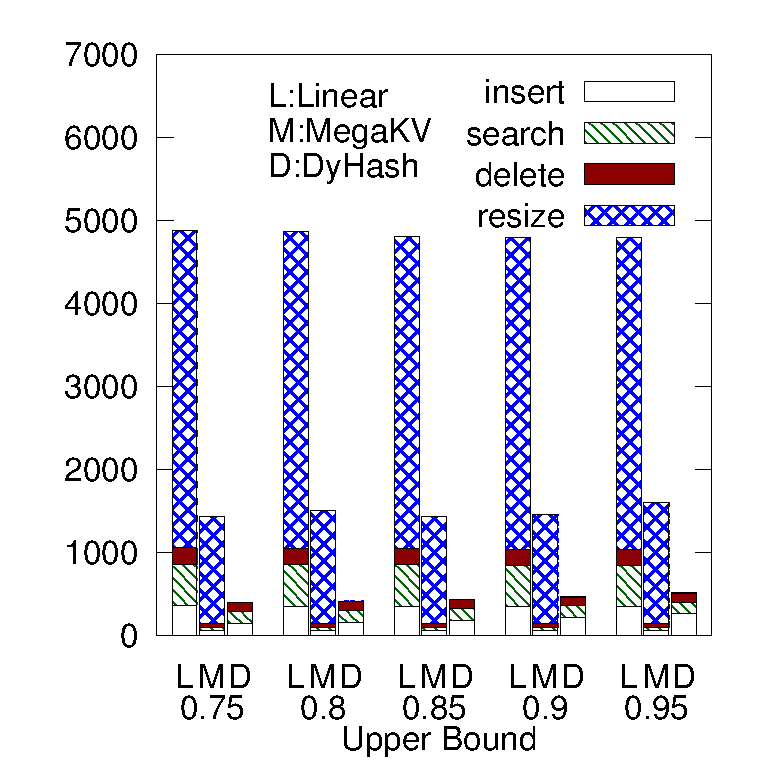
\includegraphics[width=\linewidth]{pic/dynamic/tpch/diff_upper.eps}
		\centerline{\dstpch}
	\end{minipage}
	\begin{minipage}{0.19\linewidth}\centering
		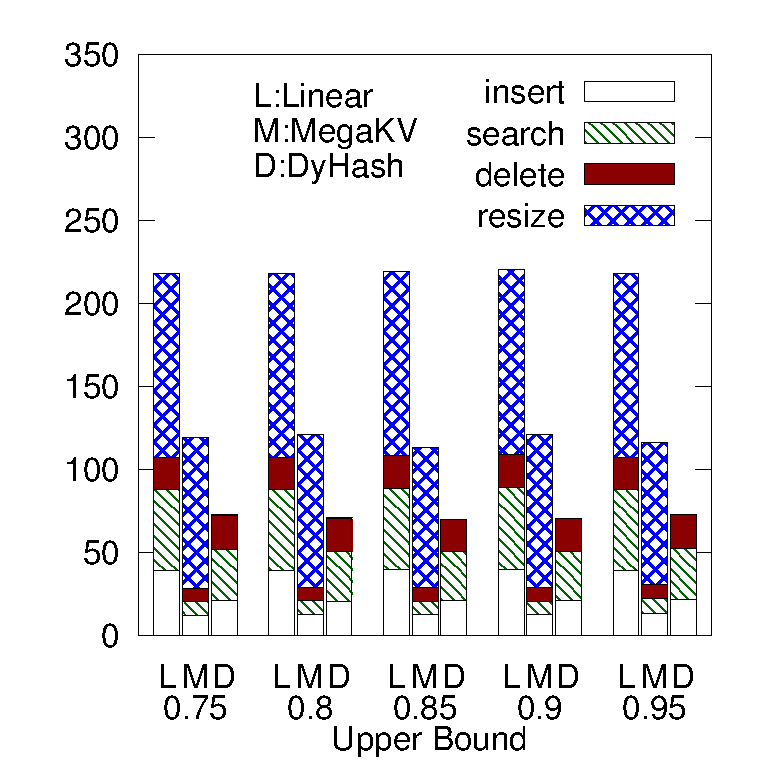
\includegraphics[width=\linewidth]{pic/dynamic/ali/diff_upper.eps}
		\centerline{\dsali}
	\end{minipage}
	\begin{minipage}{0.19\linewidth}\centering
		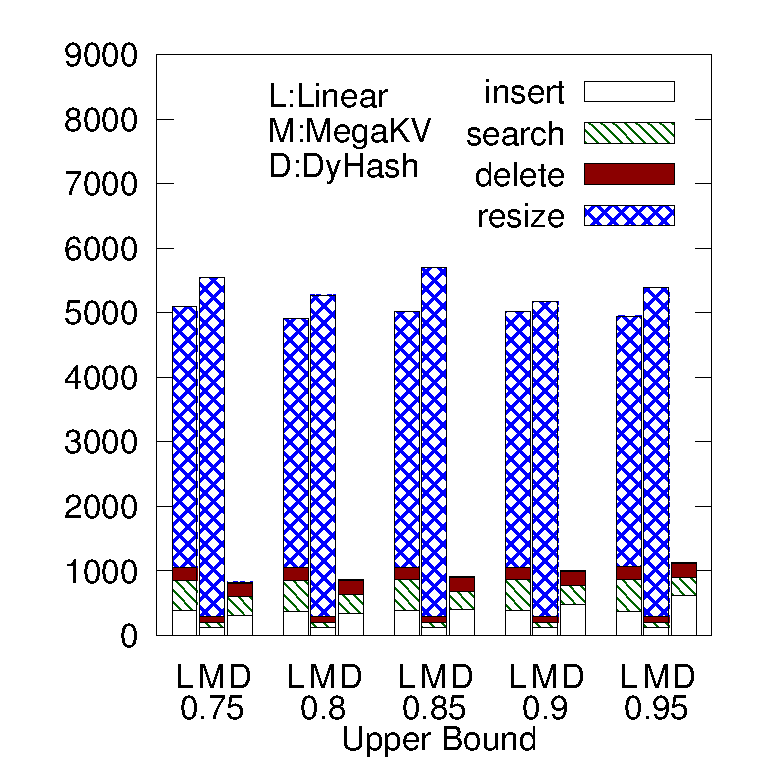
\includegraphics[width=\linewidth]{pic/dynamic/random/diff_upper.eps}
		\centerline{\dsrandom}
	\end{minipage}
	\caption{Run time for varying $\beta$.}
	\label{fig:vary-alpha-time}
\end{figure*}

\vspace{1mm}\noindent\textbf{Varying the filled factor upper bound $\beta$.}


\vspace{1mm}\noindent\textbf{Varying insert vs. delete ratio $r$.}
In Figure~\ref{fig:vary-r-time}, we report the results for varying the ratio $r$. \linear and \megakv remains inefficient as they incur expensive overheads of resizing. An interesting observation for \linear and \megakv is that there exists a sweet spot where the resizing cost is the minimal.
It is because the workload composition of insertions and deletions should be just right so that it does not trigger unnecessary upsizing or downsizing. However, in reality, the workloads could vary significantly and existing methods cannot be easily adapted while maintaining guaranteed filled factor. This has again validated the effectiveness of \voter against dynamic workloads.

\begin{figure*}[t]
	\begin{minipage}{0.19\linewidth}\centering
		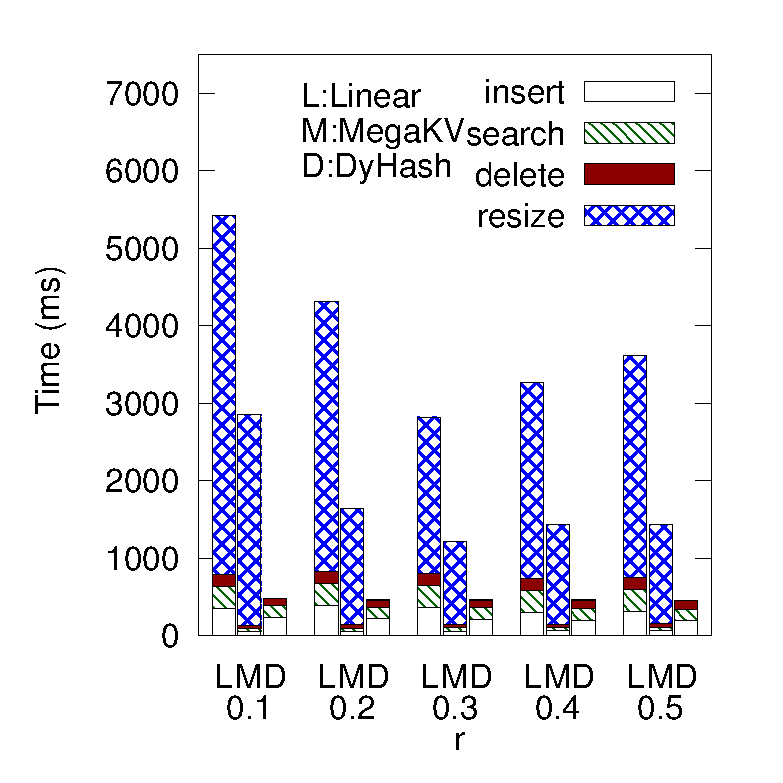
\includegraphics[width=\linewidth]{pic/dynamic/twitter/diff_r.eps}
		\centerline{\dstwitter}
	\end{minipage}
	\begin{minipage}{0.19\linewidth}\centering
		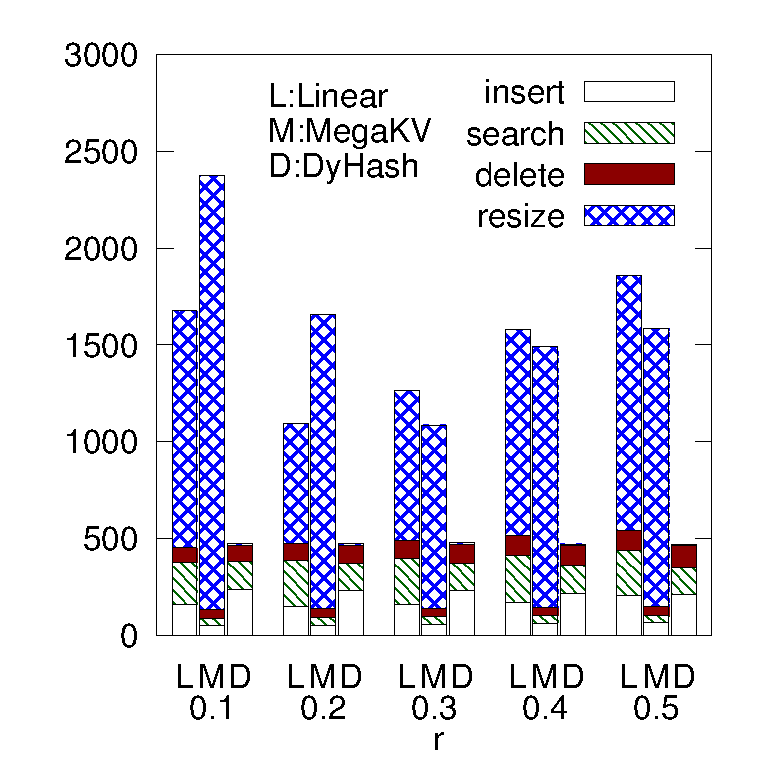
\includegraphics[width=\linewidth]{pic/dynamic/reddit/diff_r.eps}
		\centerline{\dsreddit}
	\end{minipage}
	\begin{minipage}{0.19\linewidth}\centering
		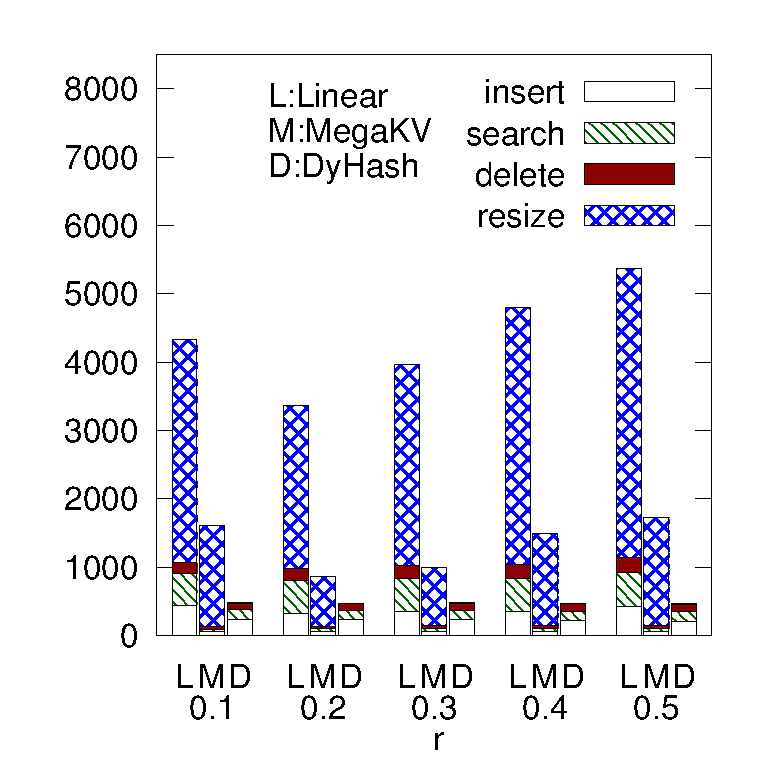
\includegraphics[width=\linewidth]{pic/dynamic/tpch/diff_r.eps}
		\centerline{\dstpch}
	\end{minipage}
	\begin{minipage}{0.19\linewidth}\centering
		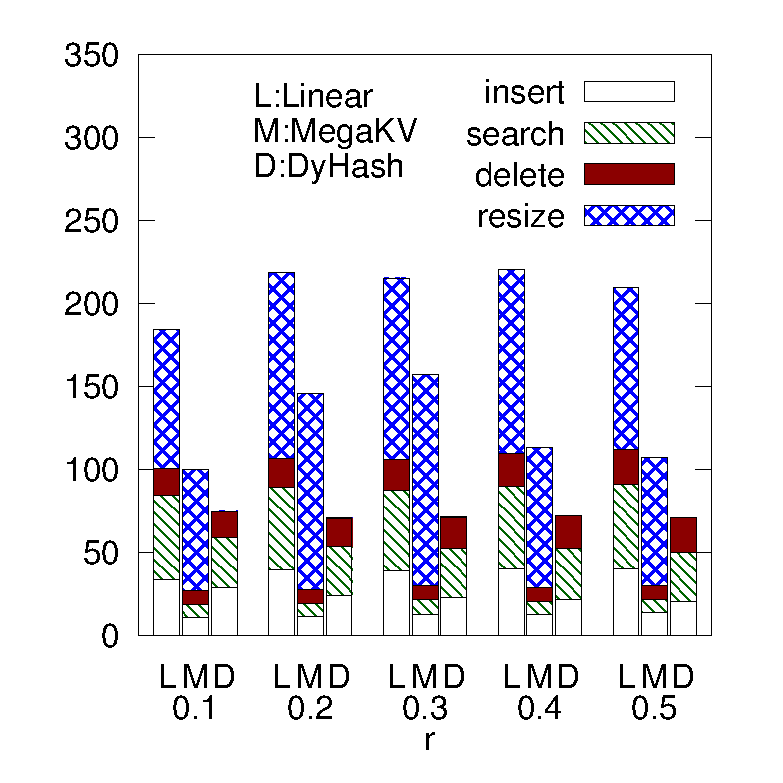
\includegraphics[width=\linewidth]{pic/dynamic/ali/diff_r.eps}
		\centerline{\dsali}
	\end{minipage}
	\begin{minipage}{0.19\linewidth}\centering
		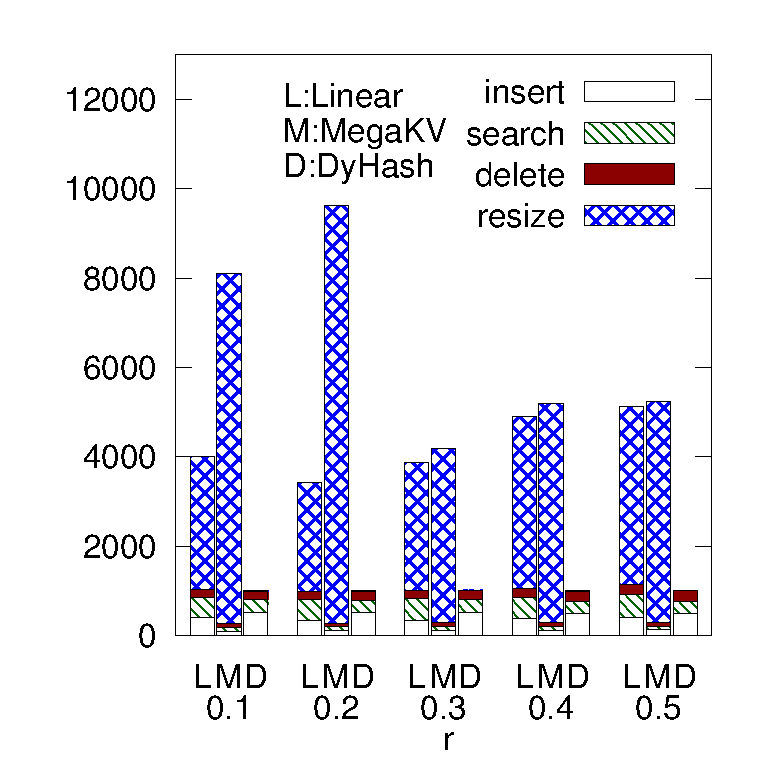
\includegraphics[width=\linewidth]{pic/dynamic/random/diff_r.eps}
		\centerline{\dsrandom}
	\end{minipage}
	\caption{Run time for varying $r$.}
	\label{fig:vary-r-time}
\end{figure*}

\vspace{1mm}\noindent\textbf{Varying the batch size.}
We have also varied the size of each processing batch. The results are reported in Figure~\ref{fig:vary-batch-size}. \voter remains the most efficient method over \linear and \megakv. It is not surprised to find that the performance of \linear and \megakv is the worst for the smallest batch size, since a fine grained processing batch triggers additional resizing for \linear and \megakv. 

\begin{figure*}[t]
	\begin{minipage}{0.19\linewidth}\centering
		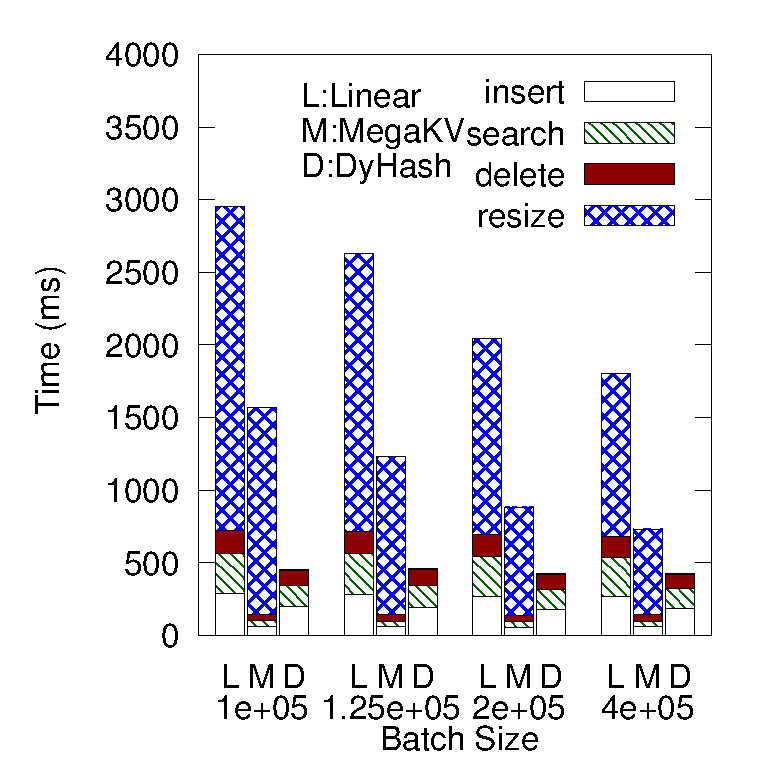
\includegraphics[width=\linewidth]{pic/dynamic/twitter/diff_batch_size.eps}
		\centerline{\dstwitter}
	\end{minipage}
	\begin{minipage}{0.19\linewidth}\centering
		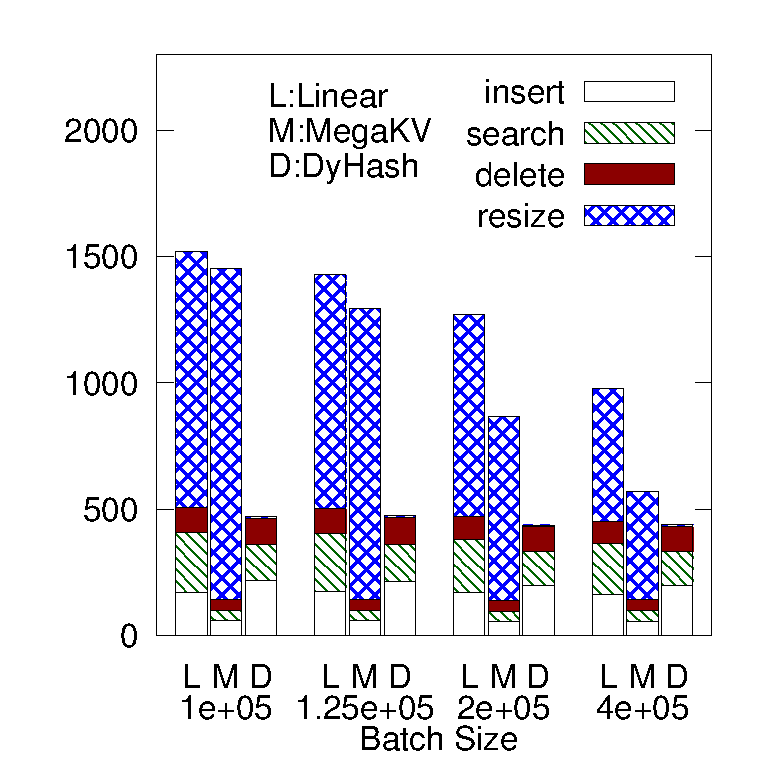
\includegraphics[width=\linewidth]{pic/dynamic/reddit/diff_batch_size.eps}
		\centerline{\dsreddit}
	\end{minipage}
	\begin{minipage}{0.19\linewidth}\centering
		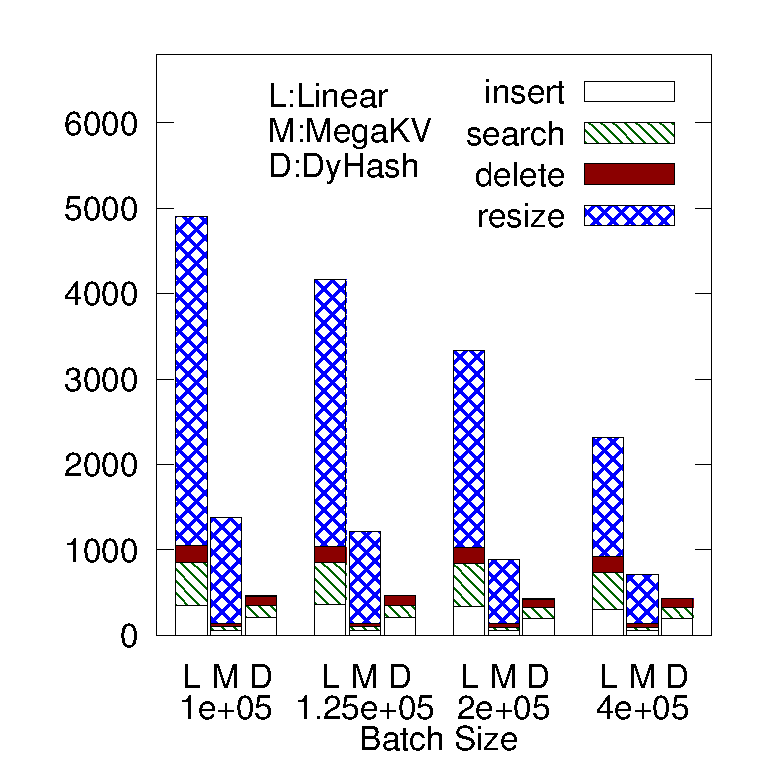
\includegraphics[width=\linewidth]{pic/dynamic/tpch/diff_batch_size.eps}
		\centerline{\dstpch}
	\end{minipage}
	\begin{minipage}{0.19\linewidth}\centering
		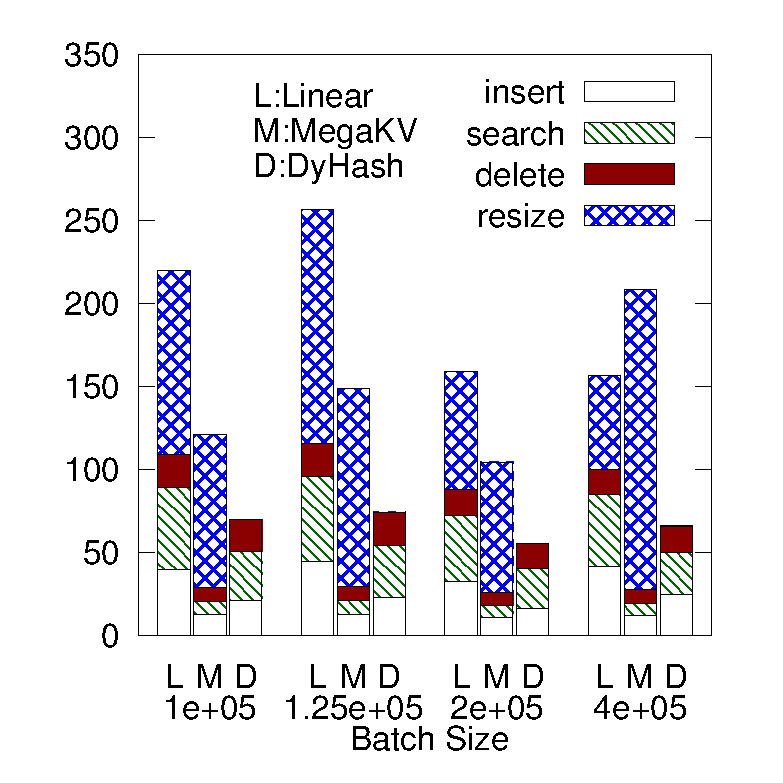
\includegraphics[width=\linewidth]{pic/dynamic/ali/diff_batch_size.eps}
		\centerline{\dsali}
	\end{minipage}
	\begin{minipage}{0.19\linewidth}\centering
		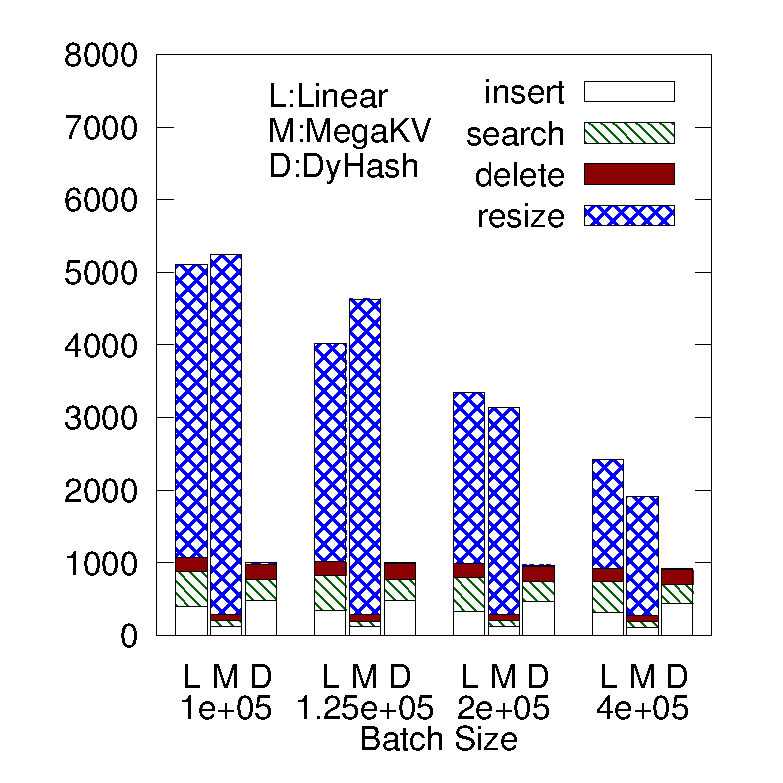
\includegraphics[width=\linewidth]{pic/dynamic/random/diff_batch_size.eps}
		\centerline{\dsrandom}
	\end{minipage}
	\caption{Run time for varying the batch size.}
	\label{fig:vary-batch-size}
\end{figure*}

\vspace{1mm}\noindent\textbf{System stability.}

\begin{figure*}[t]
	\begin{minipage}{0.19\linewidth}\centering
		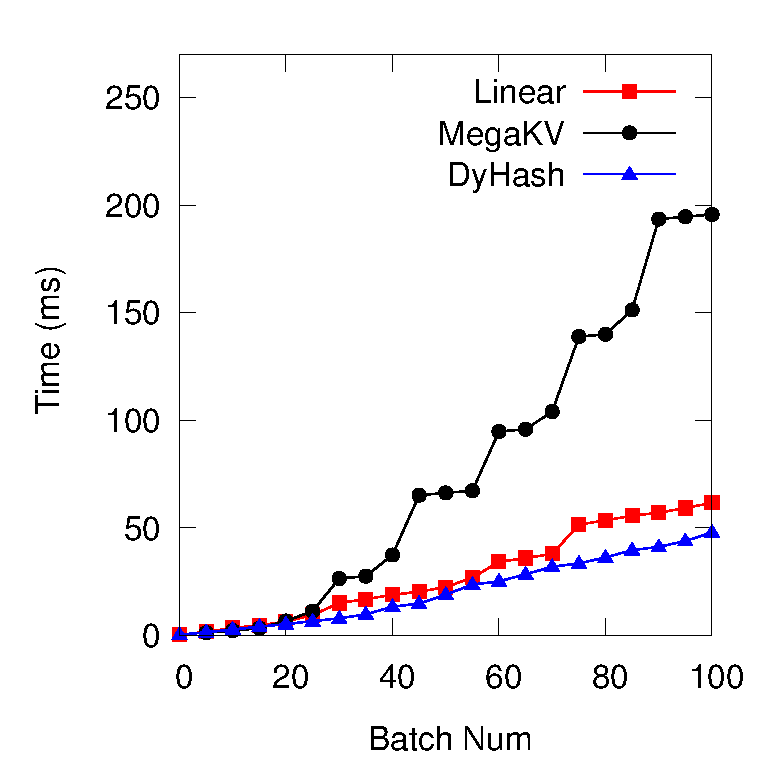
\includegraphics[width=\linewidth]{pic/dynamic-stability/dynamic-sta-twitter.eps}
		\centerline{\dstwitter}
	\end{minipage}
	\begin{minipage}{0.19\linewidth}\centering
		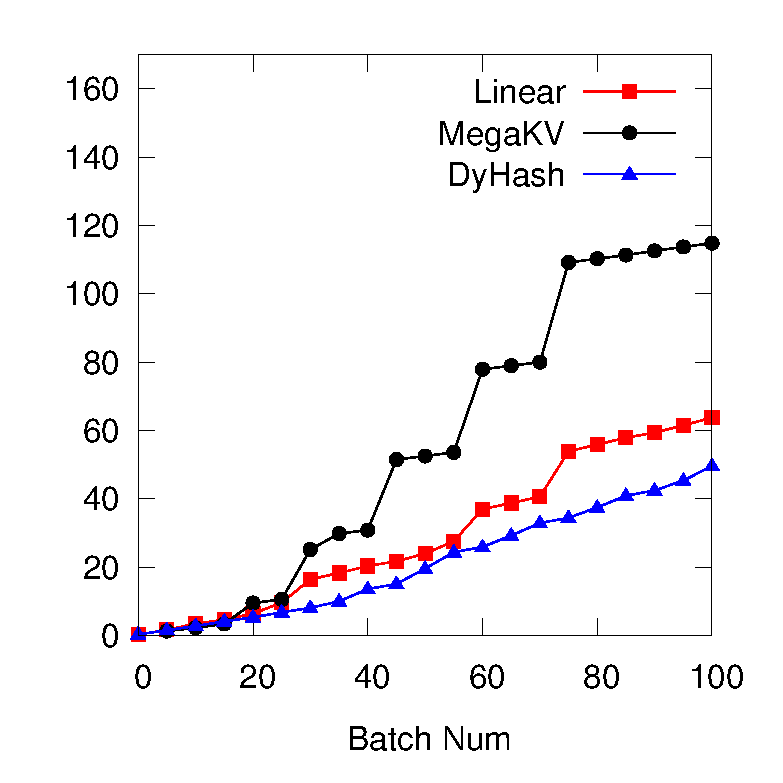
\includegraphics[width=\linewidth]{pic/dynamic-stability/dynamic-sta-reddit.eps}
		\centerline{\dsreddit}
	\end{minipage}
	\begin{minipage}{0.19\linewidth}\centering
		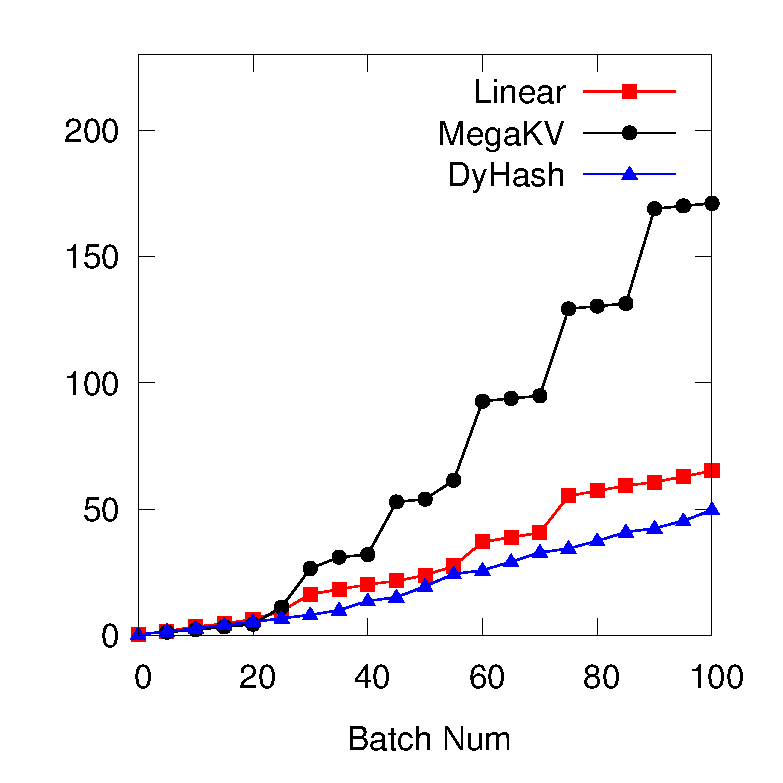
\includegraphics[width=\linewidth]{pic/dynamic-stability/dynamic-sta-tpch.eps}
		\centerline{\dstpch}
	\end{minipage}
	\begin{minipage}{0.19\linewidth}\centering
		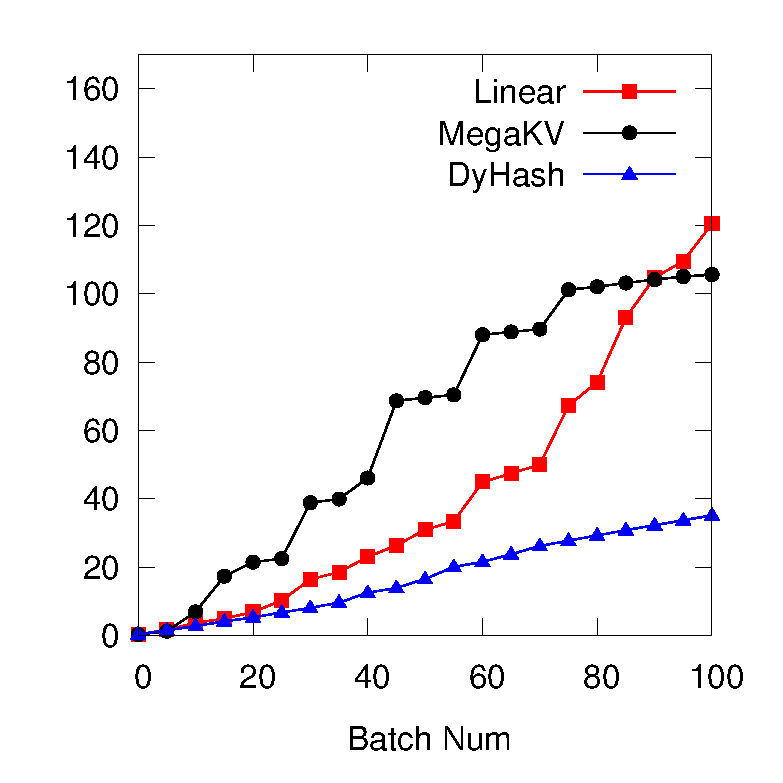
\includegraphics[width=\linewidth]{pic/dynamic-stability/dynamic-sta-ali.eps}
		\centerline{\dsali}
	\end{minipage}
	\begin{minipage}{0.19\linewidth}\centering
		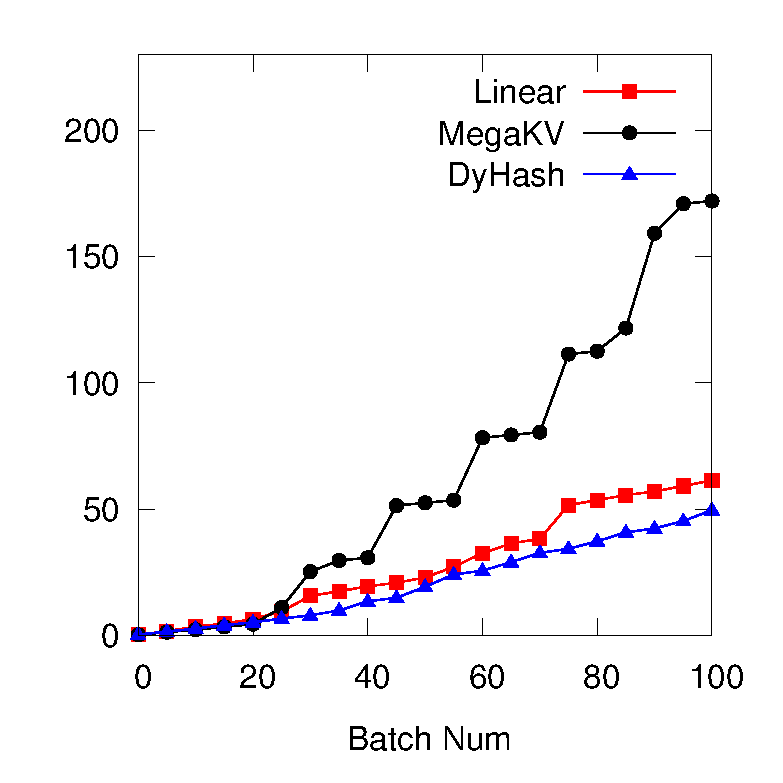
\includegraphics[width=\linewidth]{pic/dynamic-stability/dynamic-sta-random.eps}
		\centerline{\dsrandom}
	\end{minipage}
	\caption{System stability.}
	\label{fig:vary-alpha-stability}
\end{figure*}

\section{conclusion}\label{sec:con}
In this paper, we contribute a number of novel designs for dynamic hash table on GPUs. 
First, we equip the bucket-based hash table structure with a voter based coordinate scheme, 
which not only supports KV pairs with arbitrary size but also reduce the overhead of thread conflicts through the revoting mechanism. 
Second, we propose a resizing strategy that actively adjusts the table size to save GPU device memory. The resizing strategy only lock one subtable for efficient upsizing or downsizing, which allows concurrent updates to other subtables. Empirically, our proposed design achieves competitive performance against the state-of-the-art static GPU hash tables. Under the dynamic scenario, we gain up to \xxx speedups compared with baselines that uses rehashing to adjust their table size. 

 



%

\section*{Appendix}
We provide additional experiments for evaluating the static scenario performance when varying the filled factor. 
For \formal{insert}, the throughput of all approaches drop for a higher filled factor as it becomes harder to insert when the hash tables are almost filled.
For \formal{find}, all approaches except \linear has constant performance for different filled factor because they all fall into the category of cuckoo hash and has a fixed number of locations for lookups. 
Overall, \voter achieves the second best performance behind \megakv under the static scenario, which is consistent with our discussions in Section~\ref{sec:exp:static}.




%\pagebreak
\bibliographystyle{abbrv}
\bibliography{ref}
\balance

\end{document}
